\chapter{Implementation and User Interface}
		
		\section{Used technologies and tools}
		
		We have developed a mobile application for the Android operating system. The IDE of choice was Android Studio\footnote{\url{https://developer.android.com/}}. We have chosen it because it was developed by Google who are considered to be a sort of authority on Android. On the back-end we used Python\footnote{\url{https://www.python.org/}} hosted on the cloud at the site Pythonanywhere\footnote{\url{https://www.pythonanywhere.com/user/kaogrupa/}}.
		
		The database was also hosted on the aforementioned cloud. The database of choice was SQLite3\footnote{\url{https://www.sqlite.org/index.html}}. The pythonanywhere cloud offered the ability to start shell consoles and from there manage the database, as well as edit the Python back-end files. The back-end was made in Python Flask\footnote{\url{https://palletsprojects.com/p/flask/}} - a micro web framework. The cloud made the deployment and integration seamless and easy.
		
		Flask cooperates with further sub-components(as visible in the component diagram) - SQLAlchemy\footnote{\url{https://www.sqlalchemy.org/}}, Flask-JWT\footnote{\url{https://pythonhosted.org/Flask-JWT/}}, and Marshmallow\footnote{\url{https://marshmallow.readthedocs.io/en/stable/}}. SqlAlchemy is the component used for communicating with the database, JWT is used for the OAuth 2.0 implementation\footnote{\url{https://oauth.net/2/}}, and Marshmallow is used for JSON serialisation and de-serialisation. JWT = JSON Web Token.
		
		Front-end design and logic were all developed in Android Studio which provided a very convenient IDE --> code-generation and assistance was of great help, as well as the ability to edit XML files through a GUI instead of only the classical text editing. The application can be deployed and/or debugged on the mobile device by connecting it to the PC/Mac that has Android Studio running with the application code loaded into it. This has provided the basis for smooth application development and testing.
		
		Team communication was at first achieved using the Whatsapp application.\footnote{\url{https://www.whatsapp.com//}}. This worked at first, but has since proven itself to not provide satisfactory level of organisation and communication features. Therefore it was replaced with Slack\footnote{\url{https://slack.com/}} - where multiple threads and channels have made organisation and project overview much easier. What's more, a Slack bot and tasks have further increased the productivity and organisation.
		
		The version control system used was Git\footnote{\url{https://git-scm.com/}}. The most important branches were: master, dev, and devdoc. The application code was put on the dev branch, while the documentation resided on the devdoc branch. Before turning the application in, branched would be merged to the main branch --> the master branch. 
		
		The software used for documentation were: LaTeX\footnote{\url{https://www.latex-project.org/}} and Astah UML\footnote{\url{http://astah.net/}}. For LaTeX, we were provided with a template which greatly helped with LaTeX understanding and documentation writing. Astah UML was used for drawing diagrams and ha proven to be very accessible, intuitive, and satisfying to use.
		
		\eject 
	
		\section{Testing}
	
			
			\subsection{Component Testing - JUnit}
			
			We have tested the utility and some core logic classes. One test is made to deliberately fail. The code and the test results follow.
			
			First, the successful test:
			\begin{lstlisting}
package com.hfad.organizationofthefestival;

import com.hfad.organizationofthefestival.festival.Event.CreateEventActivity;
import com.hfad.organizationofthefestival.festival.Festival;
import com.hfad.organizationofthefestival.leader.Leader;
import com.hfad.organizationofthefestival.login.Login;
import com.hfad.organizationofthefestival.worker.JobApplyActivity;
import com.hfad.organizationofthefestival.worker.JobProfileActivity;
import com.hfad.organizationofthefestival.worker.Specialization;

import org.junit.Test;

import java.lang.reflect.Array;
import java.time.DateTimeException;
import java.time.ZoneId;
import java.time.ZonedDateTime;
import java.time.format.DateTimeParseException;
import java.util.ArrayList;
import java.util.List;

import static org.junit.Assert.*;

/**
* Example local unit test, which will execute on the development machine (host).
*
* @see <a href="http://d.android.com/tools/testing">Testing documentation</a>
*/
public class SuccessfulTests {
	
	Login testLogin = new Login("marko22", "");
	Login goodTestLogin = new Login("validMarko", "goodPass");
	
	@Test
	public void correctLogin() {
		
		assertEquals("marko22", testLogin.getUsername());
	}
	
	@Test
	public void isValidTest() {
		assertFalse(testLogin.isValid());
		assertTrue(goodTestLogin.isValid());
	}
	
	@Test
	public void specializationsToStringsTest(){
		List<Specialization> specializationsList = new ArrayList<>();
		
		Specialization toAdd1 = new Specialization("Writing JUnit tests");
		Specialization toAdd2 = new Specialization("Debugging");
		Specialization toAdd3 = new Specialization("Drinking alcoholic beverages");
		
		specializationsList.add(toAdd1);
		specializationsList.add(toAdd2);
		specializationsList.add(toAdd3);
		
		JobProfileActivity testJPA = new JobProfileActivity();
		List<String> actualStringList = testJPA.specializationsToStrings(specializationsList);
		
		List<String> expectedStringList = new ArrayList<>();
		expectedStringList.add("Writing JUnit tests");
		expectedStringList.add("Debugging");
		expectedStringList.add("Drinking alcoholic beverages");
		
		assertEquals(expectedStringList, actualStringList);
		
		// Let's test a mismatch
		specializationsList.clear();
		toAdd1 = new Specialization("Vacuuming");
		toAdd2 = new Specialization("Floor cleaning");
		toAdd3 = new Specialization("Desk cleaning");
		Specialization toAdd4 = new Specialization("Stage lights management");
		Specialization toAdd5 = new Specialization("Music");
		
		specializationsList.add(toAdd1);
		specializationsList.add(toAdd2);
		specializationsList.add(toAdd3);
		specializationsList.add(toAdd4);
		specializationsList.add(toAdd5);
		
		actualStringList = testJPA.specializationsToStrings(specializationsList);
		assertNotEquals(expectedStringList, actualStringList);
	}
	
	@Test
	public void parseDateTimeTest(){
		JobApplyActivity JAATest = new JobApplyActivity();
		
		String testDateTime = "2019.07.07 03:14:22";
		int year = 2019;
		int month = 7;
		int day = 7;
		int hour = 3;
		int minute = 14;
		int second = 22;
		
		ZonedDateTime actualZonedDateTime = ZonedDateTime.of(year, month, day, hour, minute, second, 0, ZoneId.systemDefault());
		ZonedDateTime expectedZonedDateTime = JAATest.parseDateTime(testDateTime);
		assertEquals(expectedZonedDateTime, actualZonedDateTime);
		
		// Let's try something that wouldn't work
		assertThrows(NumberFormatException.class, () -> {JAATest.parseDateTime("WRONG");});
		
		// Another good example
		testDateTime = "1000.01.01 03:14:22";
		year = 1000;
		month = 1;
		day = 1;
		hour = 3;
		minute = 14;
		second = 22;
		
		actualZonedDateTime = ZonedDateTime.of(year, month, day, hour, minute, second, 0, ZoneId.systemDefault());
		expectedZonedDateTime = JAATest.parseDateTime(testDateTime);
		assertEquals(expectedZonedDateTime, actualZonedDateTime);
		
		// 30.2 shouldn't exist
		assertThrows(DateTimeException.class, () -> {JAATest.parseDateTime("2019.30.02 03:14:22");});
		
		// Mismatch dates
		testDateTime = "1000.01.02 03:14:22";
		year = 1000;
		month = 1;
		day = 1;
		hour = 3;
		minute = 14;
		second = 22;
		
		actualZonedDateTime = ZonedDateTime.of(year, month, day, hour, minute, second, 0, ZoneId.systemDefault());
		expectedZonedDateTime = JAATest.parseDateTime(testDateTime);
		assertNotEquals(expectedZonedDateTime, actualZonedDateTime);
	}
	
	@Test
	public void convertTimeTest(){
		int year = 2019;
		int month = 7;
		int day = 7;
		int hour = 3;
		int minute = 14;
		int second = 22;
		ZonedDateTime expectedZDT = ZonedDateTime.of(
		year, month, day, hour, minute, second, 0, ZoneId.systemDefault()
		);
		// First a proper one
		
		CreateEventActivity CEATest = new CreateEventActivity();
		
		String expectedZDTString = "2019-07-07T03:14:00.000+0000";
		String actualZDTString = CEATest.convertTime("03:14", "07.07.2019.");
		assertEquals(expectedZDTString, actualZDTString);
		
		// Another example - a bit older but still checks out
		expectedZDTString = "0768-01-01T00:00:00.000+0000";
		actualZDTString = CEATest.convertTime("00:00", "01.01.0768.");
		assertEquals(expectedZDTString, actualZDTString);
		
		// Now let's do a bad example - MARGINAL CASE
		// 3 digit year?
		assertThrows(DateTimeParseException.class, () -> {CEATest.convertTime("00:00", "01.01.768");});
		
		// What about normal years, but single-digit minutes?
		assertThrows(DateTimeParseException.class, () -> {CEATest.convertTime("1:00", "01.01.2020");});
		
		// What about single-digit months or days?
		assertThrows(DateTimeParseException.class, () -> {CEATest.convertTime("00:00", "1.01.2021");});
	}
	
	@Test
	public void getFestivalTest() {
		Leader testLeader = new Leader(0, "testLeader",
		"123", "Testo", "Testen"
		, "SAMPLE-IMAGE", "09819819"
		, "test@test.com", 1, 0);
		
		// Let's first test an empty list
		List<Festival> festivalsList = new ArrayList<>();
		testLeader.setFestivals(festivalsList);
		
		assertEquals(null, testLeader.getFestival("CoolFest"));
		// Now let's add the CoolFest
		Festival coolFest = new Festival("coolFest", "very cool"
		, "SAMPLE-LOGO", "6 oclock", "never"
		);
		festivalsList.add(coolFest);
		
		assertEquals(null, testLeader.getFestival("wut"));
		assertEquals(coolFest, testLeader.getFestival("coolFest"));
		
		// Now let's test getFestivalNames method
		// Will need more festivals
		Festival superFest = new Festival("superFest", "very cool"
		, "SAMPLE-LOGO", "6 oclock", "never"
		);
		Festival marinFest = new Festival("marinFest", "very cool"
		, "SAMPLE-LOGO", "6 oclock", "never"
		);
		Festival boatFest = new Festival("boatFest", "very cool"
		, "SAMPLE-LOGO", "6 oclock", "never"
		);
		
		festivalsList.add(superFest);
		festivalsList.add(marinFest);
		festivalsList.add(boatFest);
		List<String> expectedFestNames = new ArrayList<>();
		expectedFestNames.add("coolFest");
		expectedFestNames.add("superFest");
		expectedFestNames.add("marinFest");
		expectedFestNames.add("boatFest");
		assertEquals(expectedFestNames, testLeader.getFestivalNames());
	}
}
			\end{lstlisting}
			
			And now the test that deliberately fails!
			\begin{lstlisting}
package com.hfad.organizationofthefestival;

import com.hfad.organizationofthefestival.festival.Festival;
import com.hfad.organizationofthefestival.worker.Specialization;

import org.junit.Test;

import static org.junit.Assert.assertThrows;

public class FailingTest {

@Test
public void emptyTests(){
	// Can we make a no-name specialization?
		assertThrows(IllegalArgumentException.class, () -> {
			Specialization emptySpec = new Specialization("");
		});

	// Can we make empty Festival?
		assertThrows(IllegalArgumentException.class, () -> {
			Festival boatFest = new Festival("", "very cool"
				, "SAMPLE-LOGO", "6 oclock", "never");
		});
	}
}
			\end{lstlisting}
			
			Their results:
			\begin{figure}[H]
				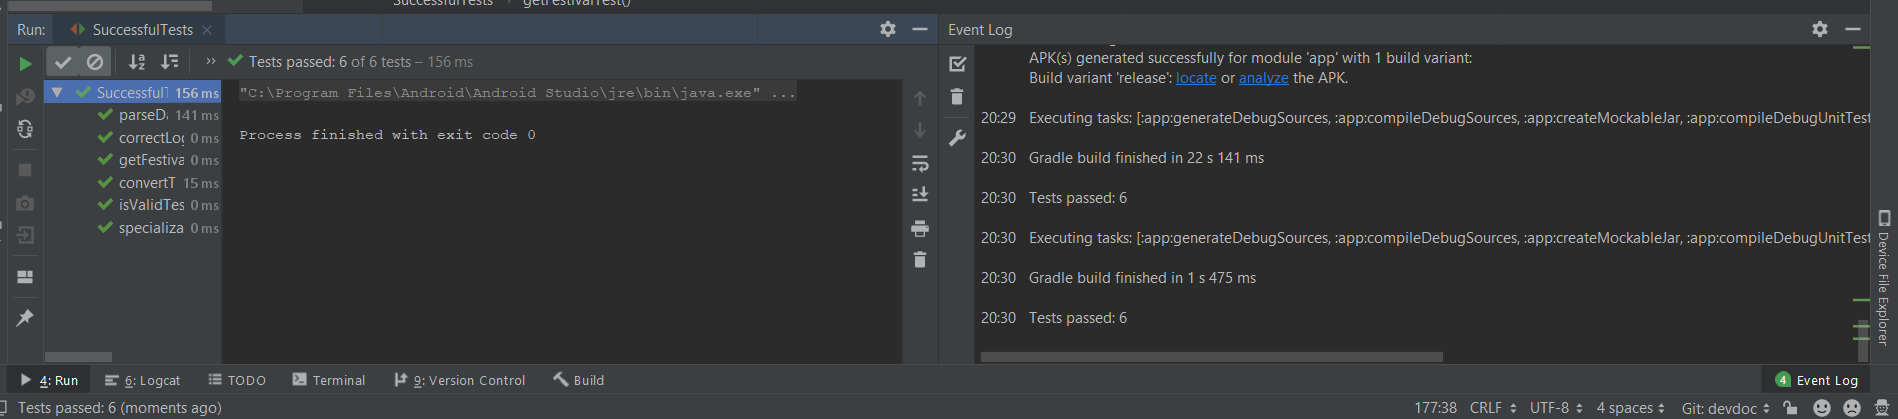
\includegraphics[width=\linewidth]{images/JUnit_1.png}
				\caption{Successful tests}
				\label{fig:junit_1}
			\end{figure}
		
			\begin{figure}[H]
				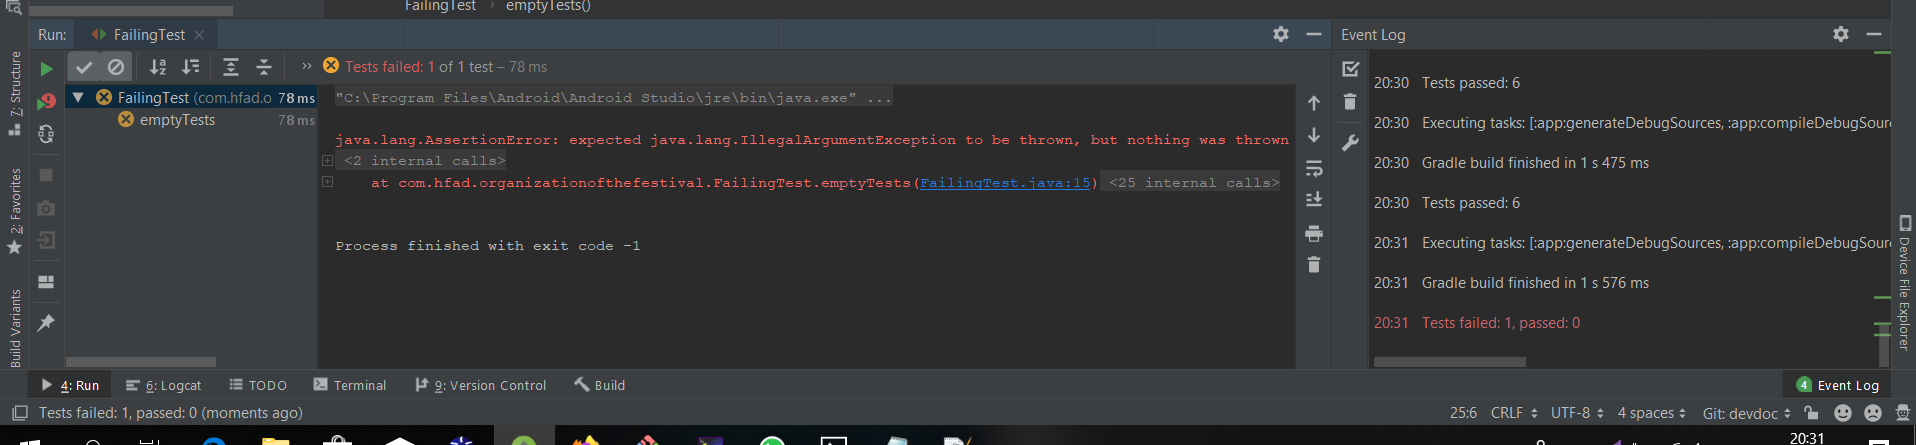
\includegraphics[width=\linewidth]{images/JUnit_2.png}
				\caption{Failing tests}
				\label{fig:junit_2}
			\end{figure}
			
			\subsection{System Testing}
			
			 \textbf{Test Scenario 1: Leader register and festival creation test}
			 Input:
			 \begin{packed_enum}
			 	\item Tap 'No account yet? Create one'.
			 	\item Input user data and chose 'Leader' from drop-down list, and Tap 'Create account'.
			 	\item Tap 'Already a member? Login'.
			 	\item Input admin user data, tap 'Login', and tap 'Accept' next to created leader, go back on login screen.
			 	\item Input created leader user data, tap 'Login', tap 'Create new festival', input festival data, tap 'Create'.
			 \end{packed_enum}
		 
		 	Expected output:
		 	\begin{packed_enum}
		 		\item Opened register screen
		 		\item Get message about successful account creation.
		 		\item Opened login screen
		 		\item Get message about successfully accepted leader.
		 		\item Get message about successfully created festival.
		 	\end{packed_enum}
	 	
	 		Actual result:
	 		\begin{packed_enum}
	 			\item Opened register screen.
	 			\item Get message about successful account creation.
	 			\item Opened login screen.
	 			\item Get message about successfully accepted leader.
	 			\item Get message about successfully created festival.
	 		\end{packed_enum}
	 		
	 		\textbf{Test Scenario 2 - Leader search test}
	 		Input:
	 		\begin{packed_enum}
	 			\item Input organizer user data, tap 'Login'
	 			\item Tap 'Search'.
	 			\item Leave empty field, tap 'Search'.
	 			\item Input 'leader007', tap 'Search'.
	 		\end{packed_enum}
	 		
	 		Expected output:
	 		\begin{packed_enum}
	 			\item Login as organizer.
	 			\item Open search screen.
	 			\item List all users.
	 			\item List only user 'leader007'.
	 		\end{packed_enum}
	 		
	 		Actual result:
	 		\begin{packed_enum}
	 			\item Login as organizer.
	 			\item Open search screen.
	 			\item List all users.
	 			\item List only user 'leader007'.
	 		\end{packed_enum}
	 		
	 		\begin{figure}[H]
	 			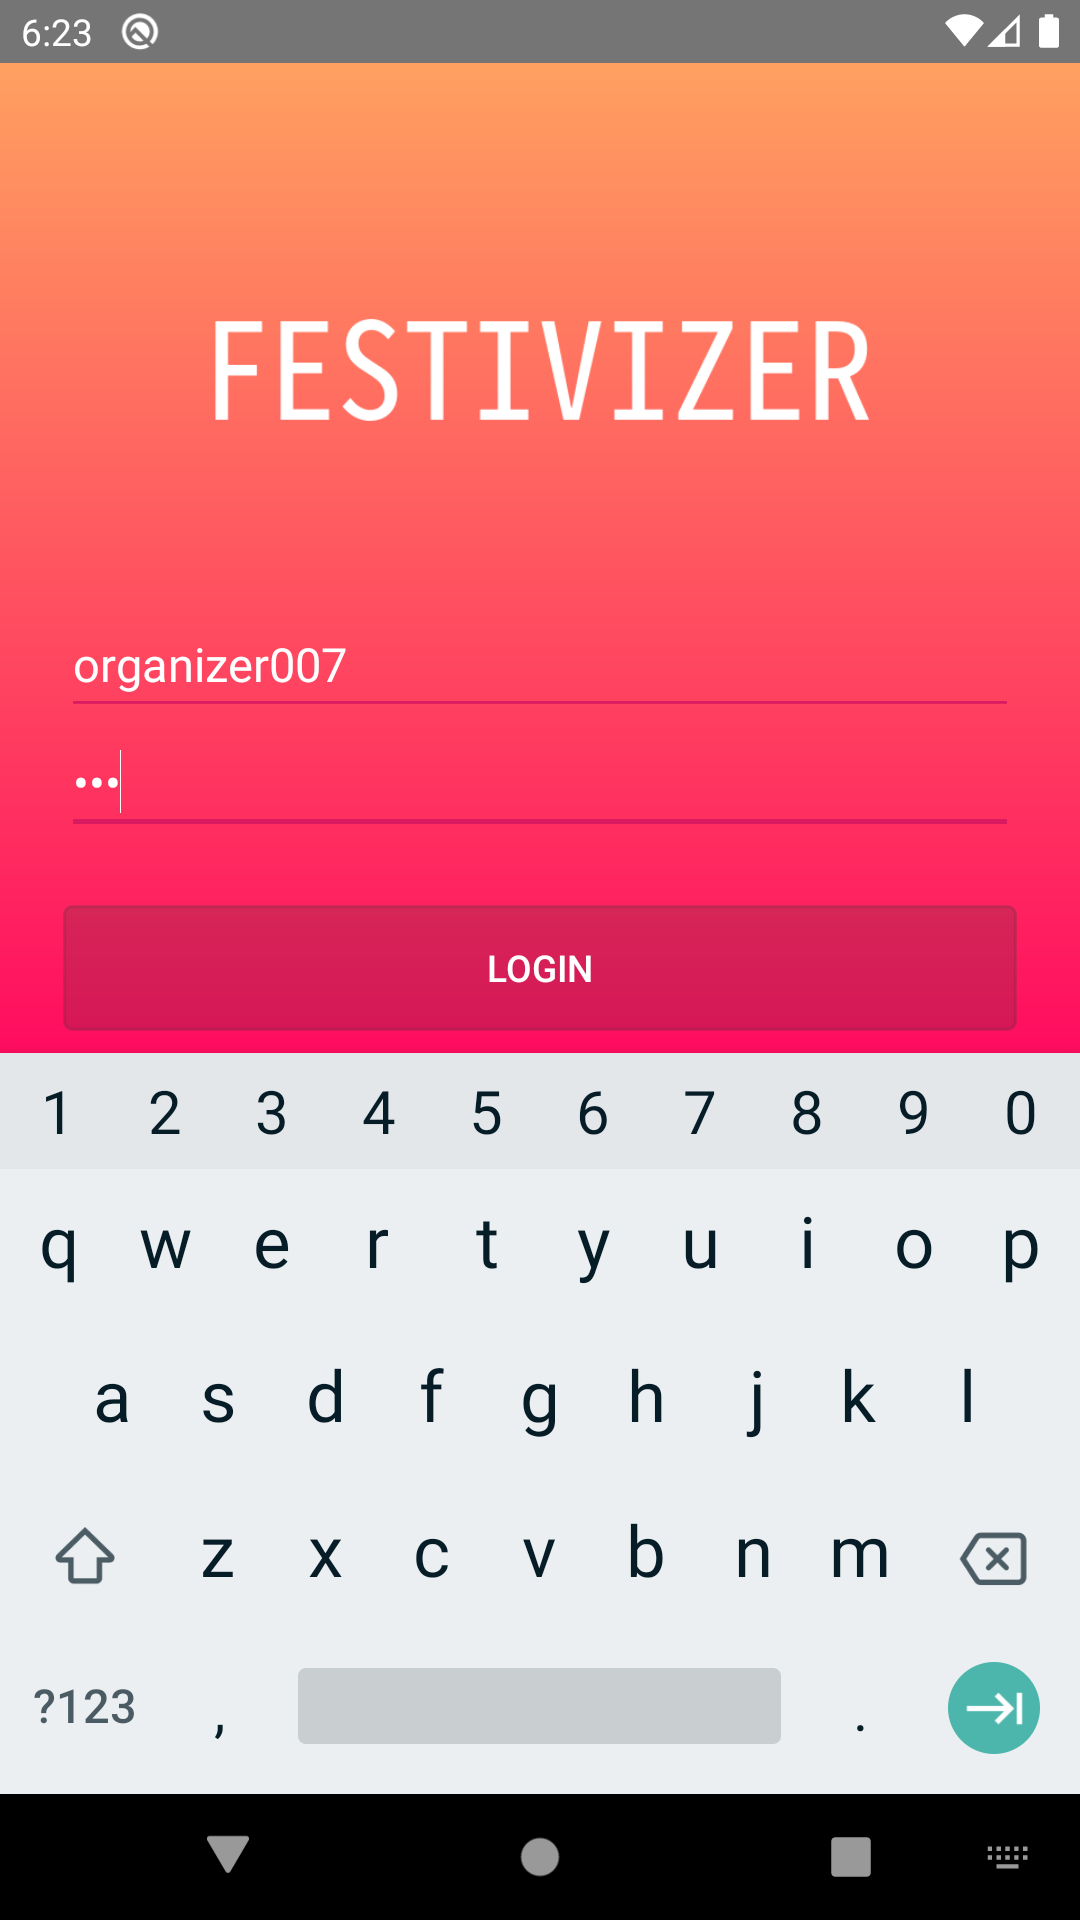
\includegraphics[width=\linewidth]{images/test_Screens/test_scenario_2-1.png}
	 			\caption{Test scenario 2}
	 			\label{fig:espresso_2_1}
	 		\end{figure}
	 		
	 		\begin{figure}[H]
	 			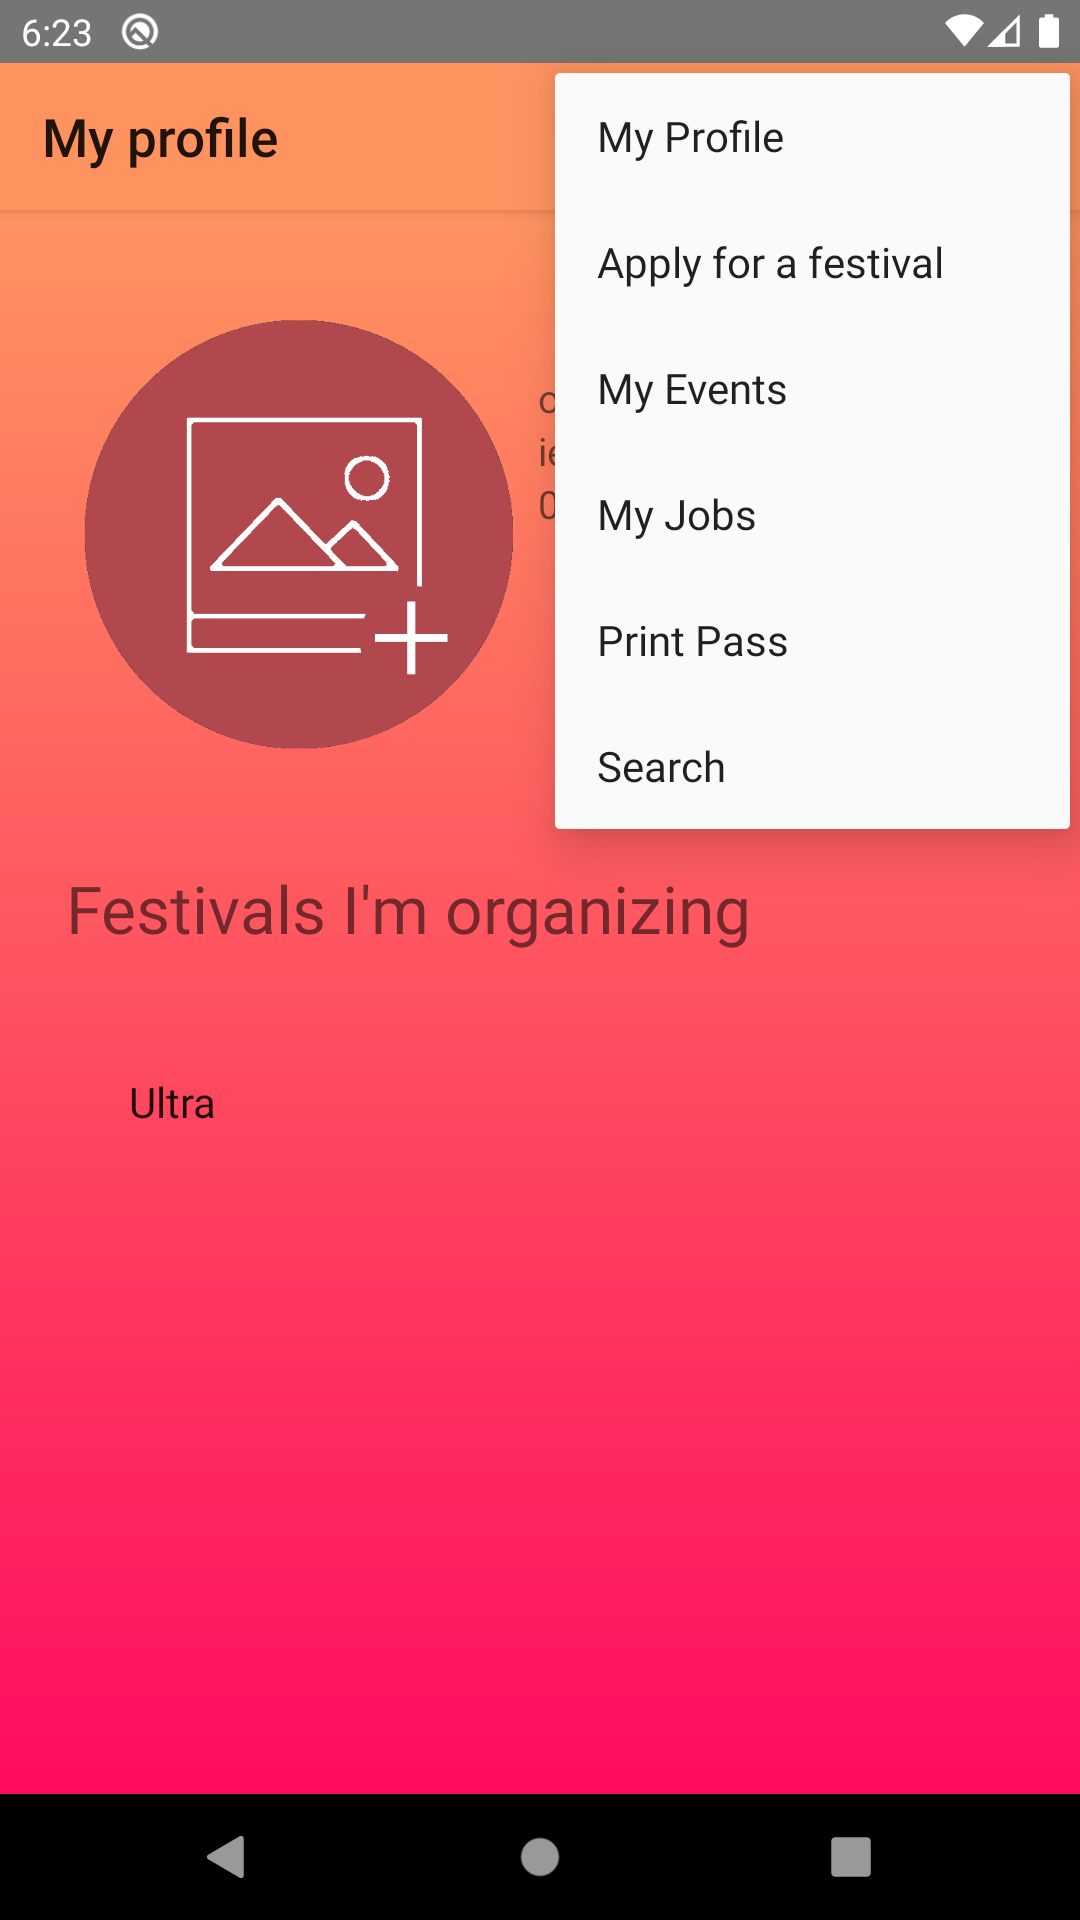
\includegraphics[width=\linewidth]{images/test_Screens/test_scenario_2-2.png}
	 			\caption{Test scenario 2}
	 			\label{fig:espresso_2_2}
	 		\end{figure}
	 		
	 		\begin{figure}[H]
	 			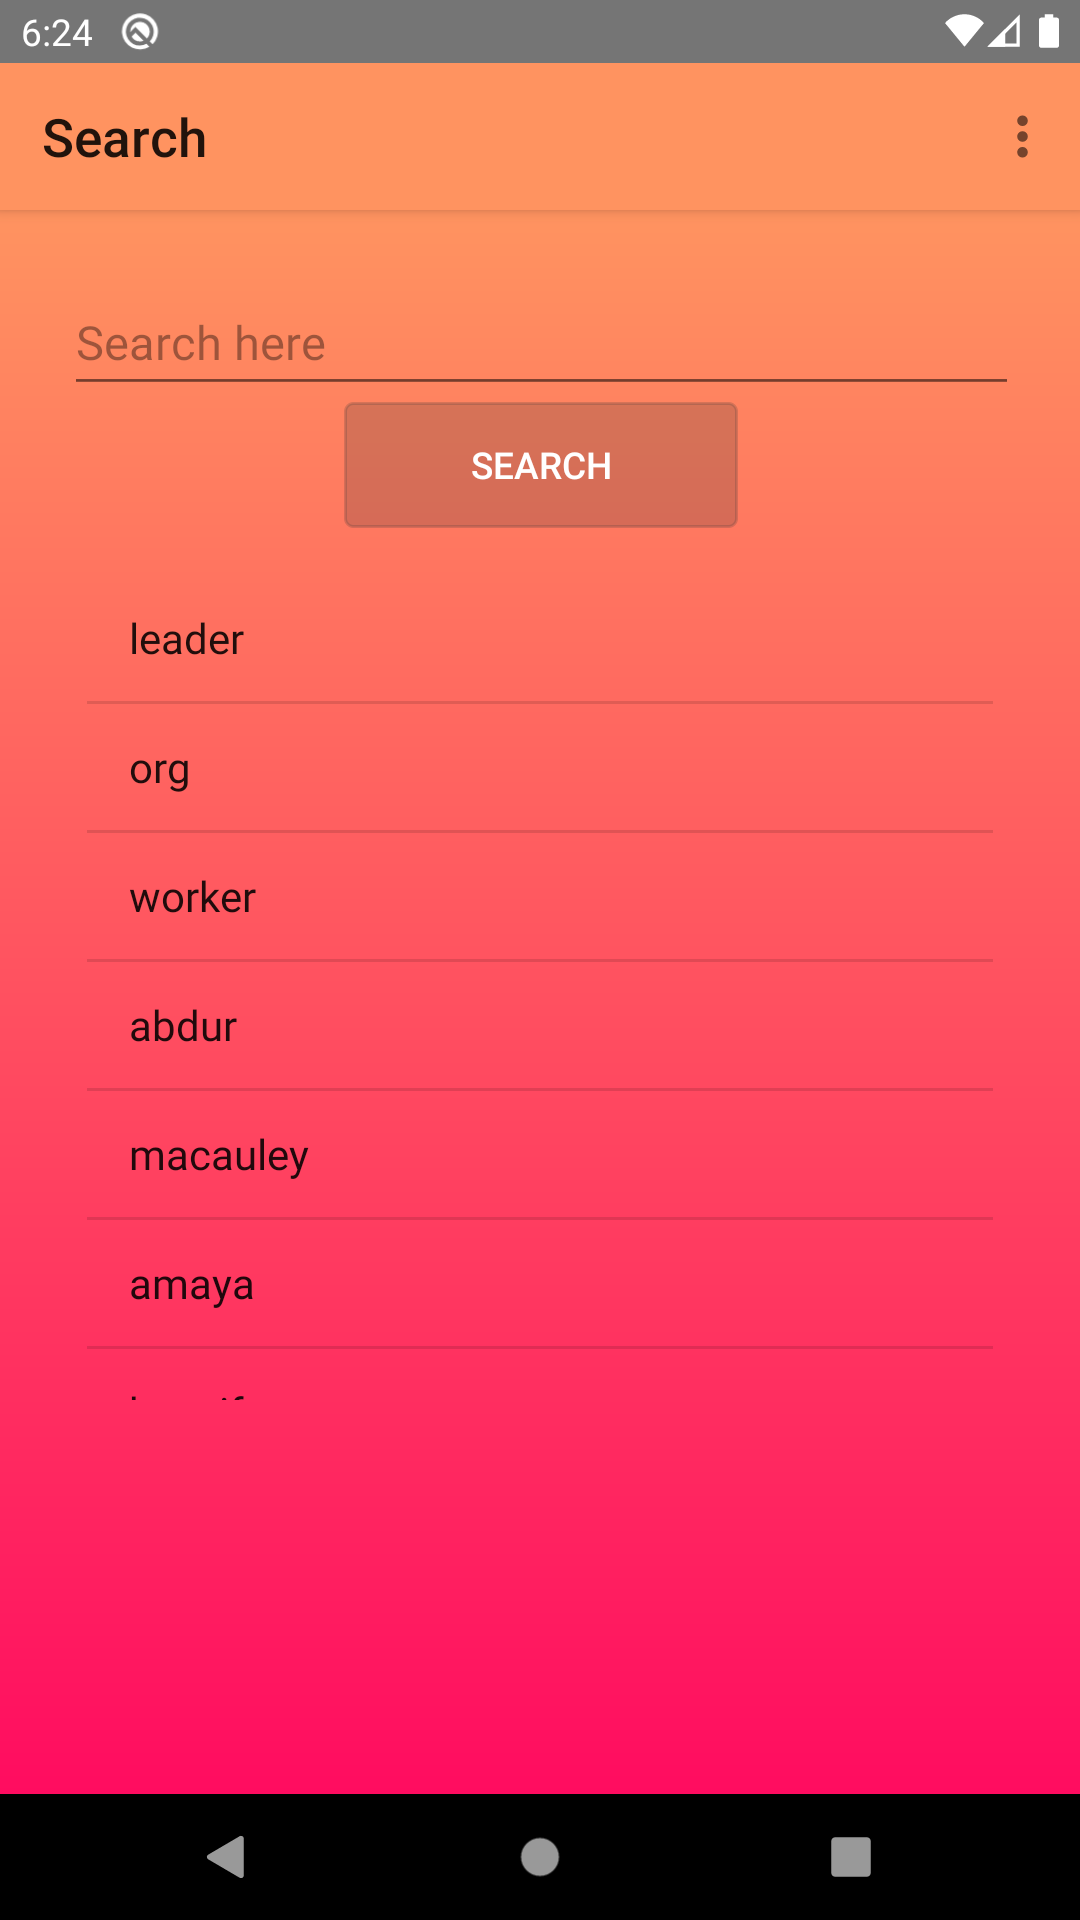
\includegraphics[width=\linewidth]{images/test_Screens/test_scenario_2-3.png}
	 			\caption{Test scenario 2}
	 			\label{fig:espresso_2_3}
	 		\end{figure}
	 		
	 		\begin{figure}[H]
	 			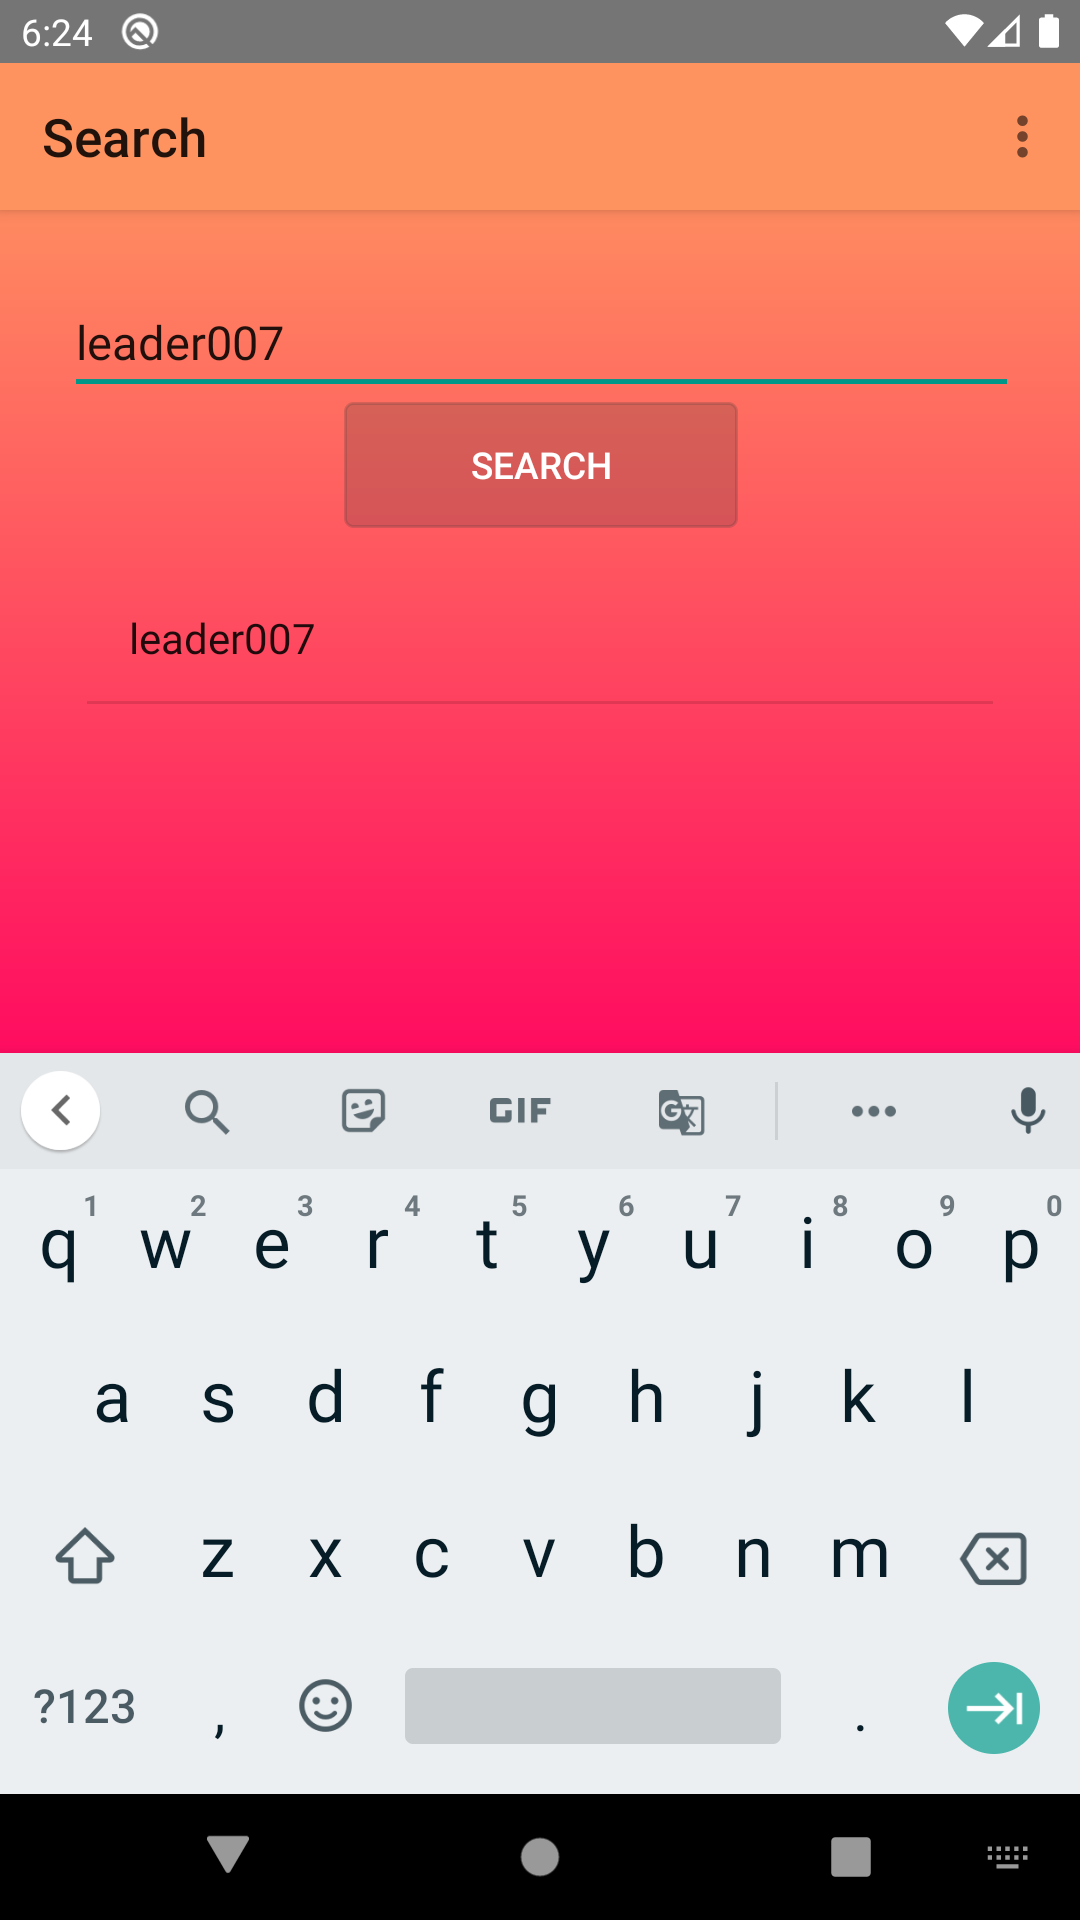
\includegraphics[width=\linewidth]{images/test_Screens/test_scenario_2-4.png}
	 			\caption{Test scenario 2}
	 			\label{fig:espresso_2_4}
	 		\end{figure}
	 		
	 		\textbf{Test Scenario 3 - Organizer job creation test}
	 		Input:
	 		\begin{packed_enum}
	 			\item Input organizer user data, tap 'Login'.
	 			\item Tap 'My events', tap some active event, tap 'New Job'.
	 			\item Input required data, tap 'Create job'.
	 		\end{packed_enum}
 		
 			Expected output:
 			\begin{packed_enum}
 				\item Login as organizer.
 				\item Open job creation screen.
 				\item Get message about successfully created job.
 			\end{packed_enum}
	 		
	 		Actual result:
	 		\begin{packed_enum}
	 			\item Login as organizer.
	 			\item Open job creation screen.
	 			\item Get message about successfully created job.
	 		\end{packed_enum}
			\eject 
			
			\textbf{Test Scenario 4 - Organizer print pass test}
			Input:
			\begin{packed_enum}
				\item Input organizer user data, tap 'Login'.
				\item Tap 'Search'.
			\end{packed_enum}
			
			Expected output:
			\begin{packed_enum}
				\item Login as organizer.
				\item Create required PDF file with pass, get message about successfully created file.
			\end{packed_enum}
			
			Actual result:
			\begin{packed_enum}
				\item Login as organizer.
				\item Loading in infinite loop. (BUG shown)
			\end{packed_enum}
		
			\begin{figure}[H]
				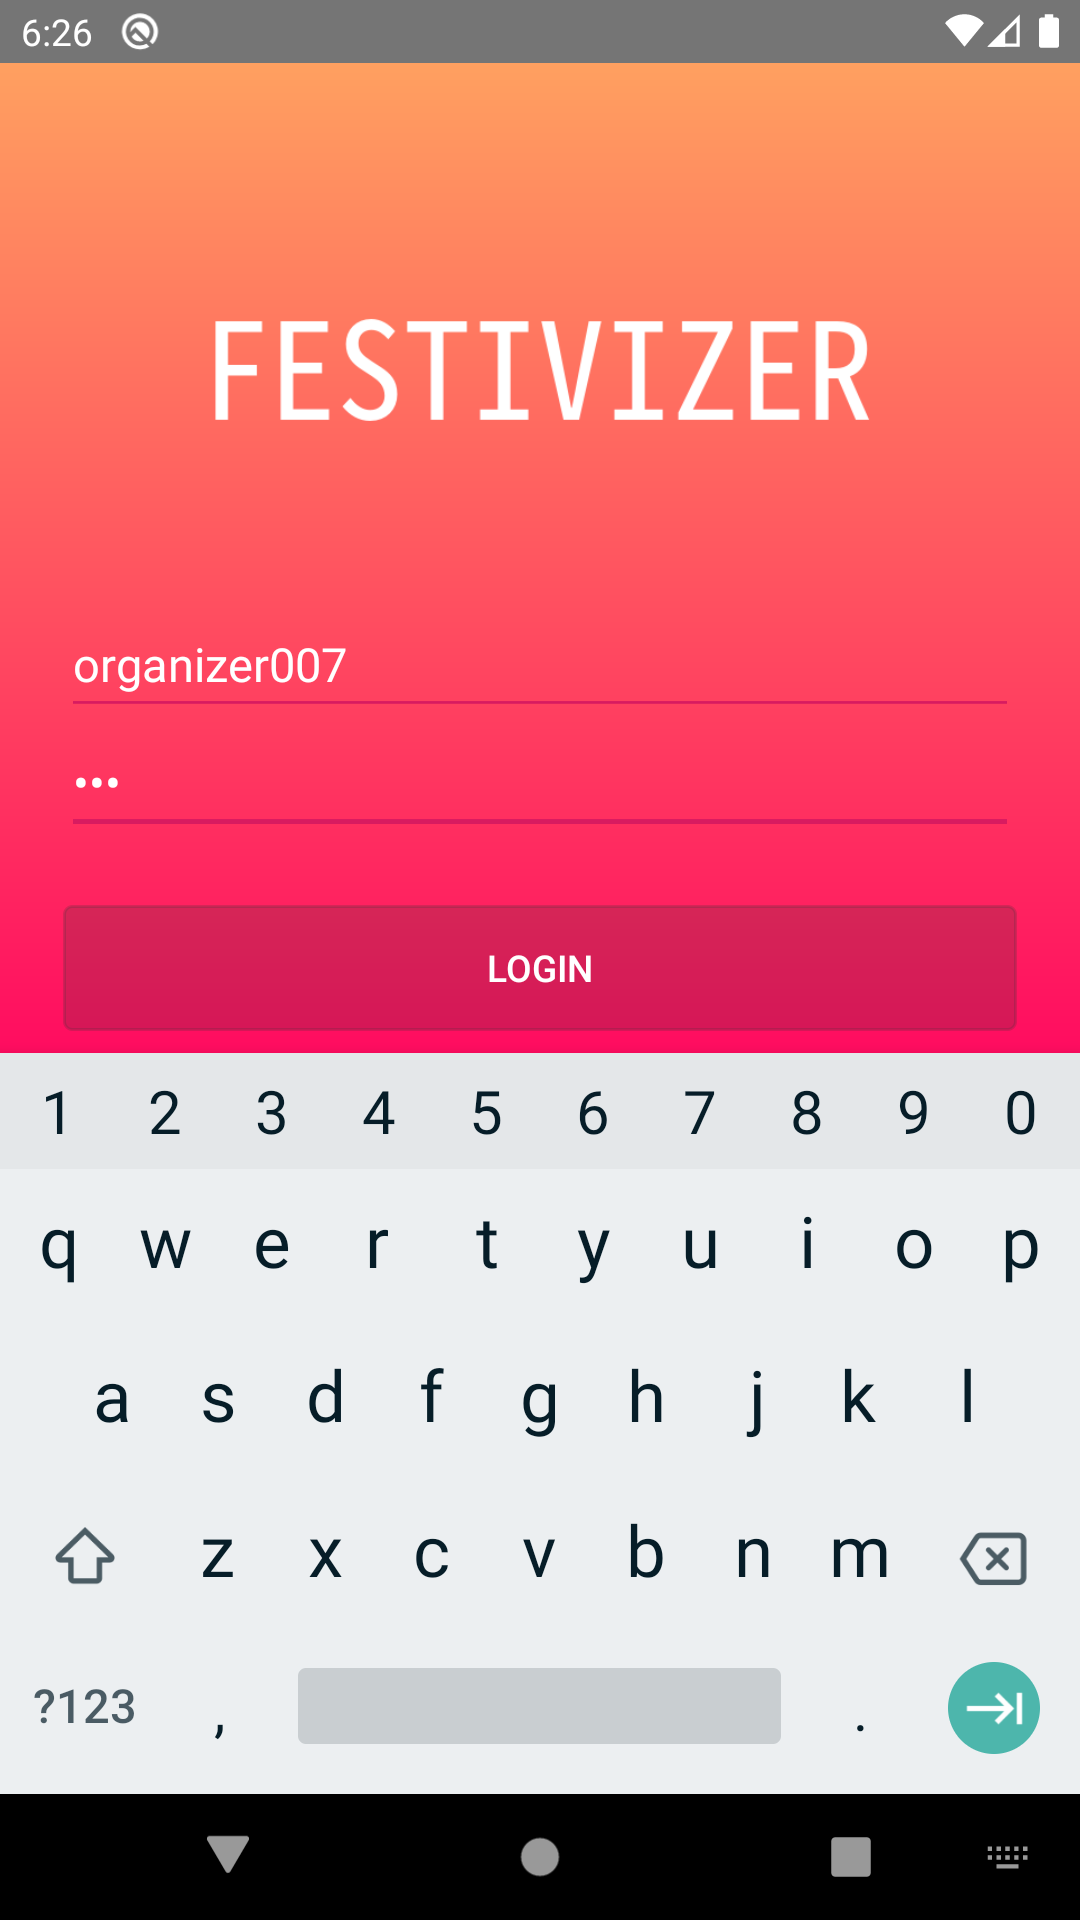
\includegraphics[width=\linewidth]{images/test_Screens/test_scenario_4-1.png}
				\caption{Test scenario 4}
				\label{fig:espresso_4_1}
			\end{figure}
			
			\begin{figure}[H]
				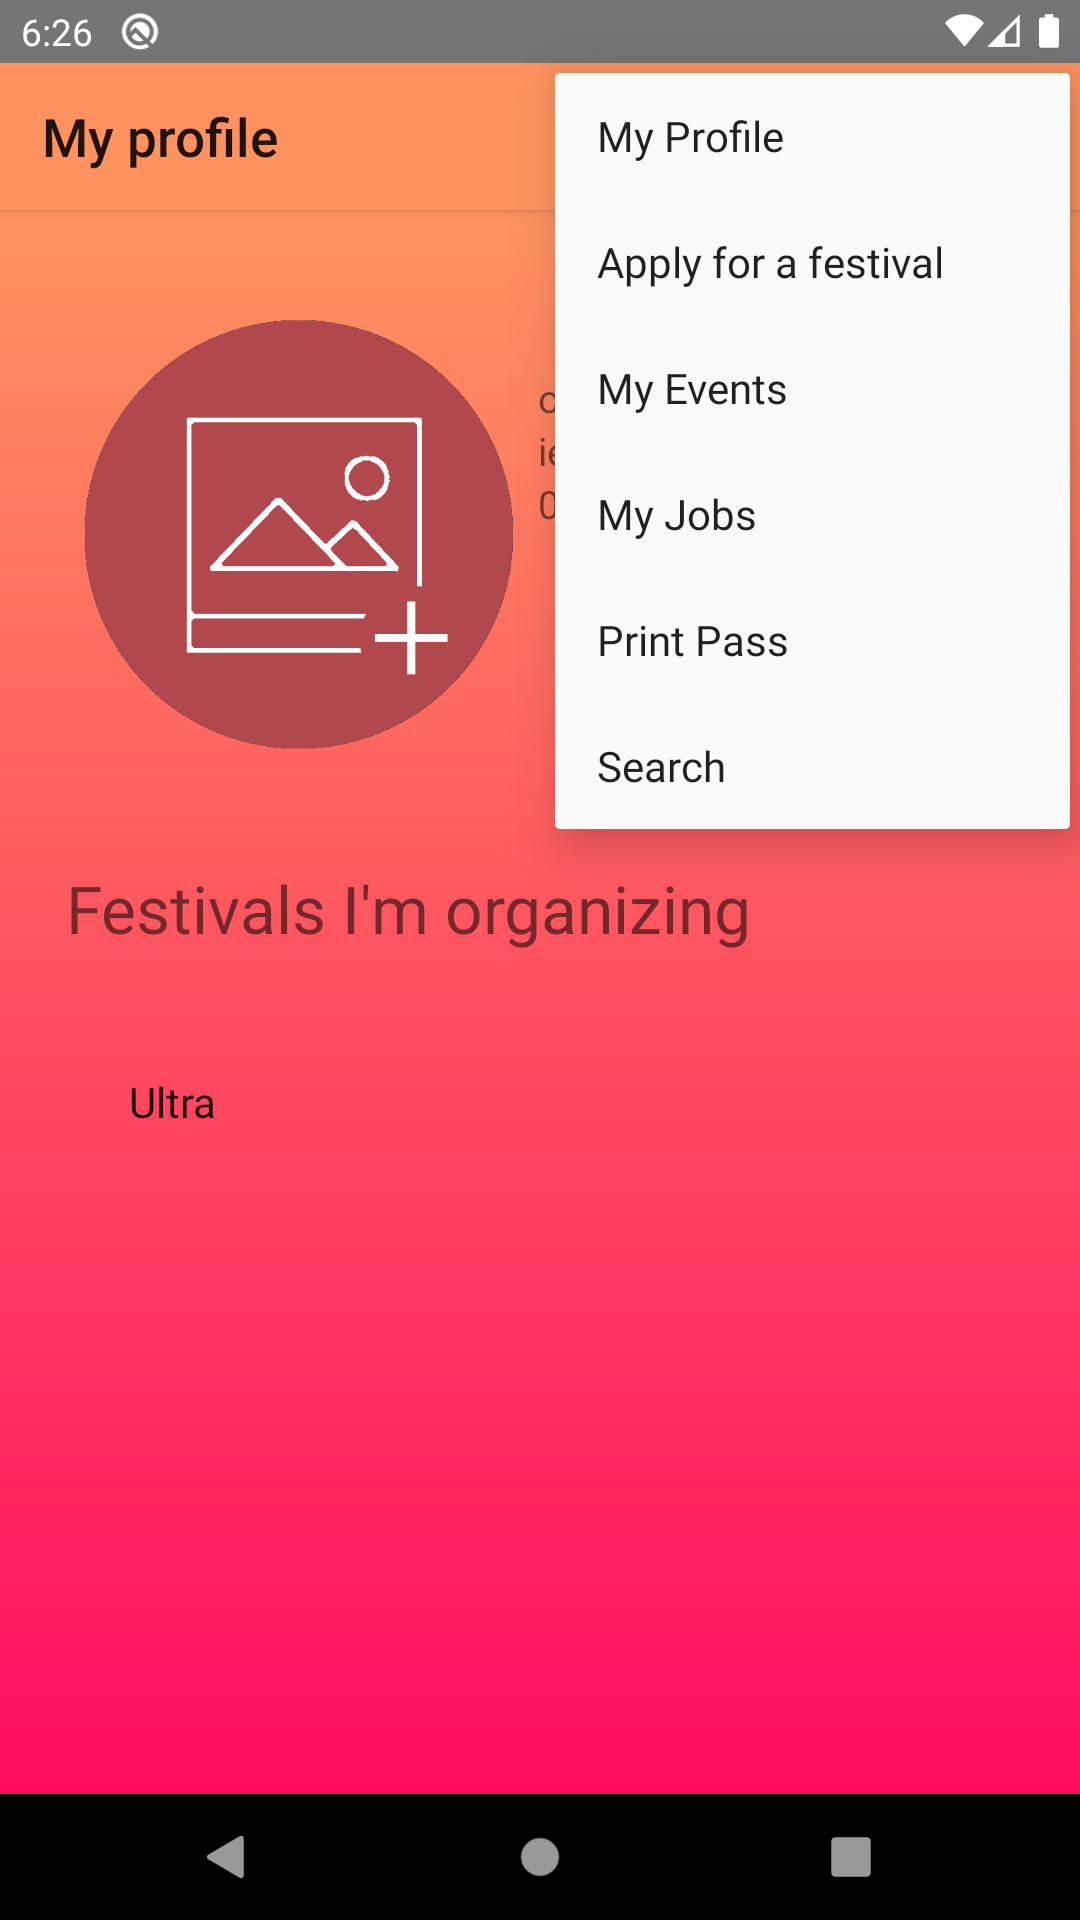
\includegraphics[width=\linewidth]{images/test_Screens/test_scenario_4-2.png}
				\caption{Test scenario 4}
				\label{fig:espresso_4_2}
			\end{figure}
			
			\begin{figure}[H]
				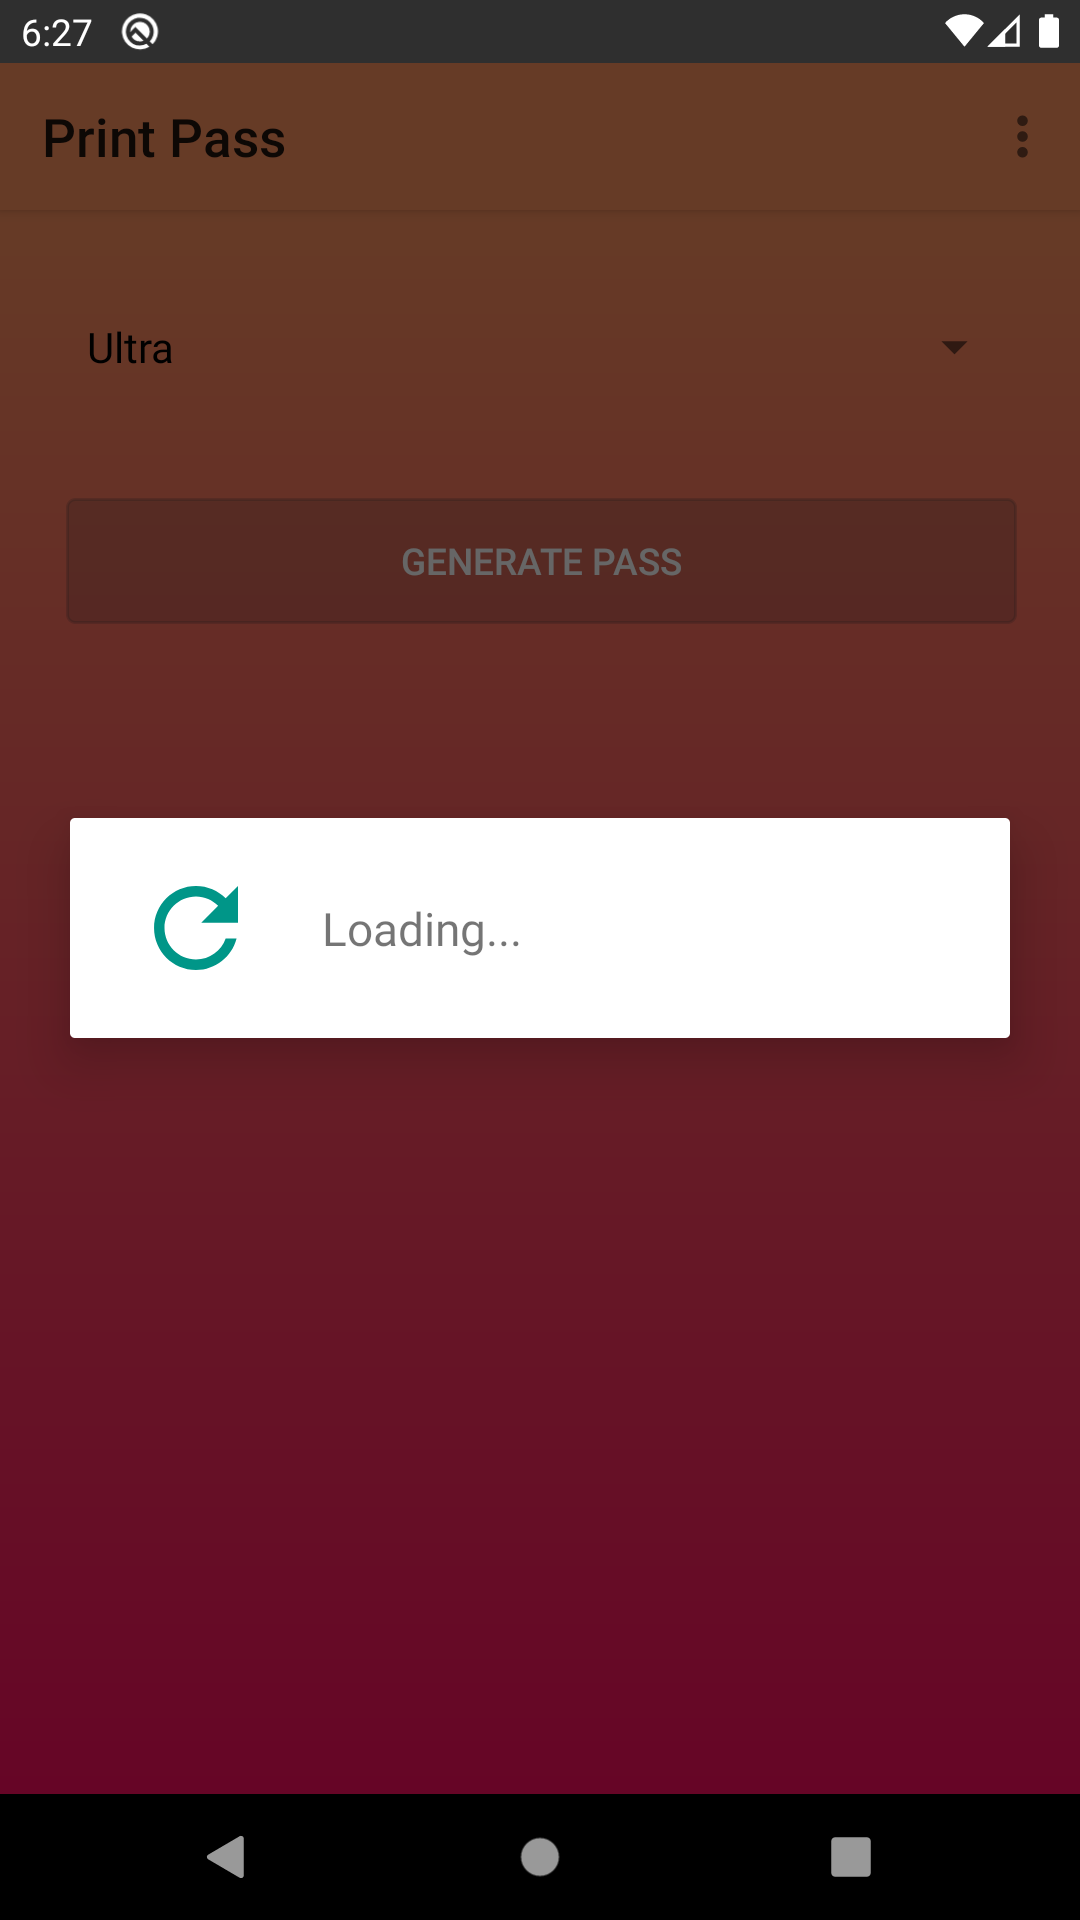
\includegraphics[width=\linewidth]{images/test_Screens/test_scenario_4-3.png}
				\caption{Test scenario 4}
				\label{fig:espresso_4_3}
			\end{figure}
		
			\textbf{Test Scenario 5 - Organizer print pass test}
			Input:
			\begin{packed_enum}
				\item Tap 'No account yet? Create one'.
				\item Input user data and chose 'Organizer' from drop-down list, and Tap 'Create account'.
				\item Tap 'Already a member? Login'.
				\item Input organizer user data, tap 'Login'.
				\item Tap 'Apply for a festival', tap on some festival or festivals.
			\end{packed_enum}
			
			Expected output:
			\begin{packed_enum}
				\item Opened register screen.
				\item Get message about successful account creation.
				\item Opened login screen.
				\item Login as organizer.
				\item Get message about successfully applied for a festival, and see tick next to selected festivals.
			\end{packed_enum}
			
			Actual result:
			\begin{packed_enum}
				\item Opened register screen.
				\item Get message about successful account creation.
				\item Opened login screen.
				\item Login as organizer.
				\item Get message about successfully applied for a festival, and see tick next to selected festivals.
			\end{packed_enum}
			
			\begin{figure}[H]
				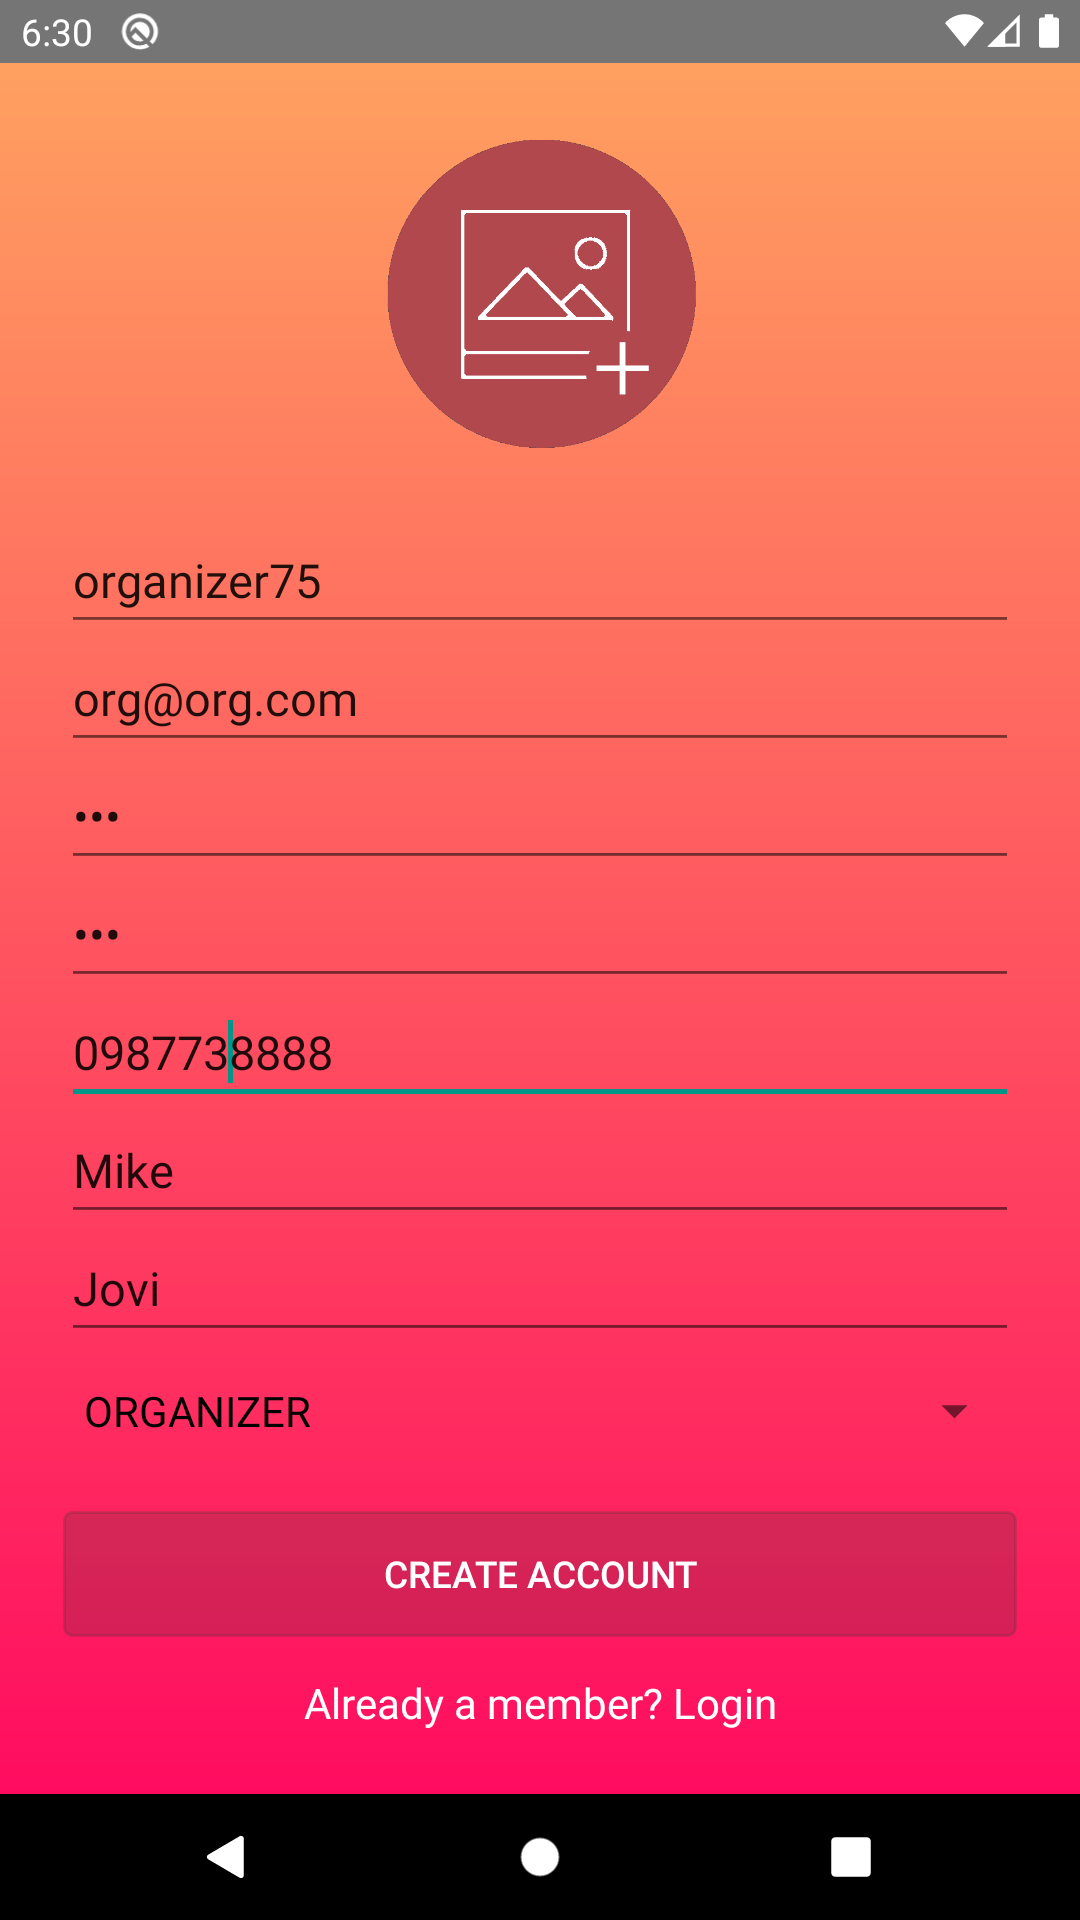
\includegraphics[width=\linewidth]{images/test_Screens/test_scenario_5-1.png}
				\caption{Test scenario 5}
				\label{fig:espresso_5_1}
			\end{figure}
			
			\begin{figure}[H]
				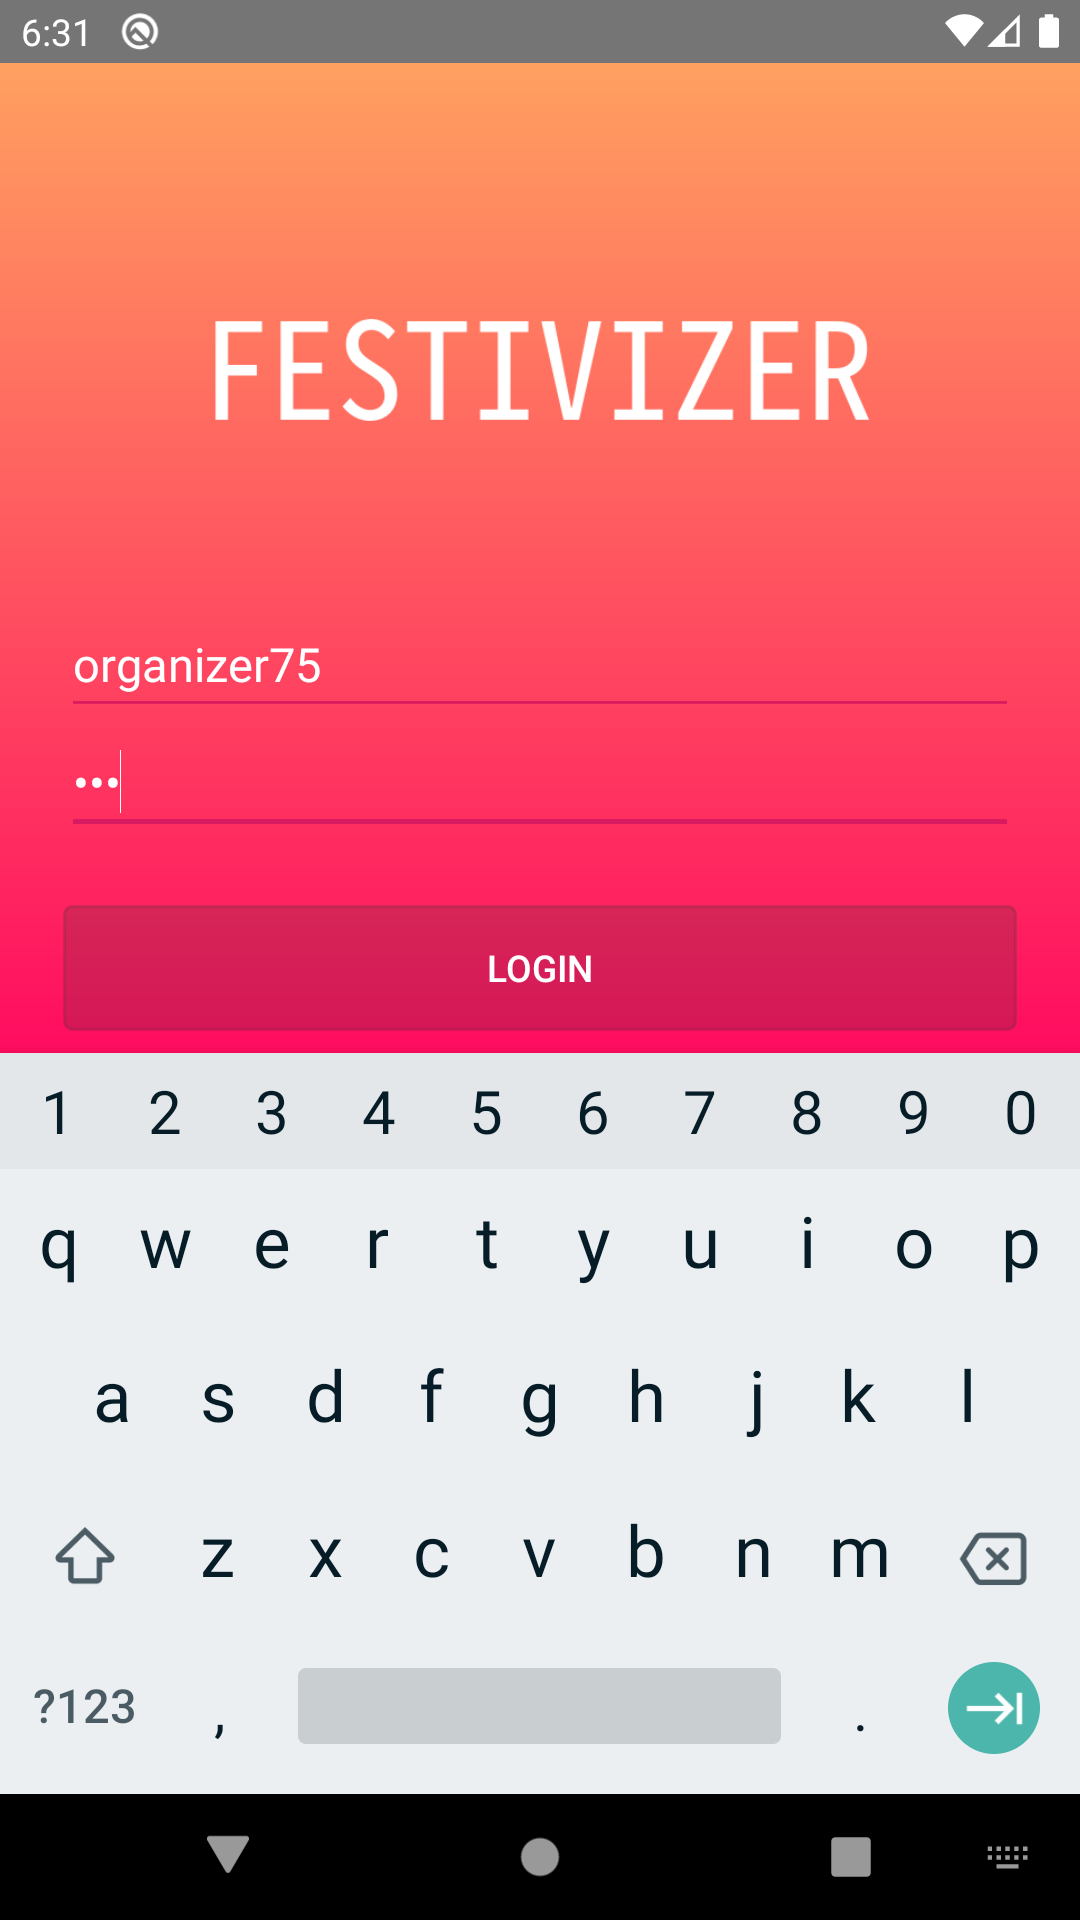
\includegraphics[width=\linewidth]{images/test_Screens/test_scenario_5-2.png}
				\caption{Test scenario 5}
				\label{fig:espresso_5_2}
			\end{figure}
		
			\begin{figure}[H]
				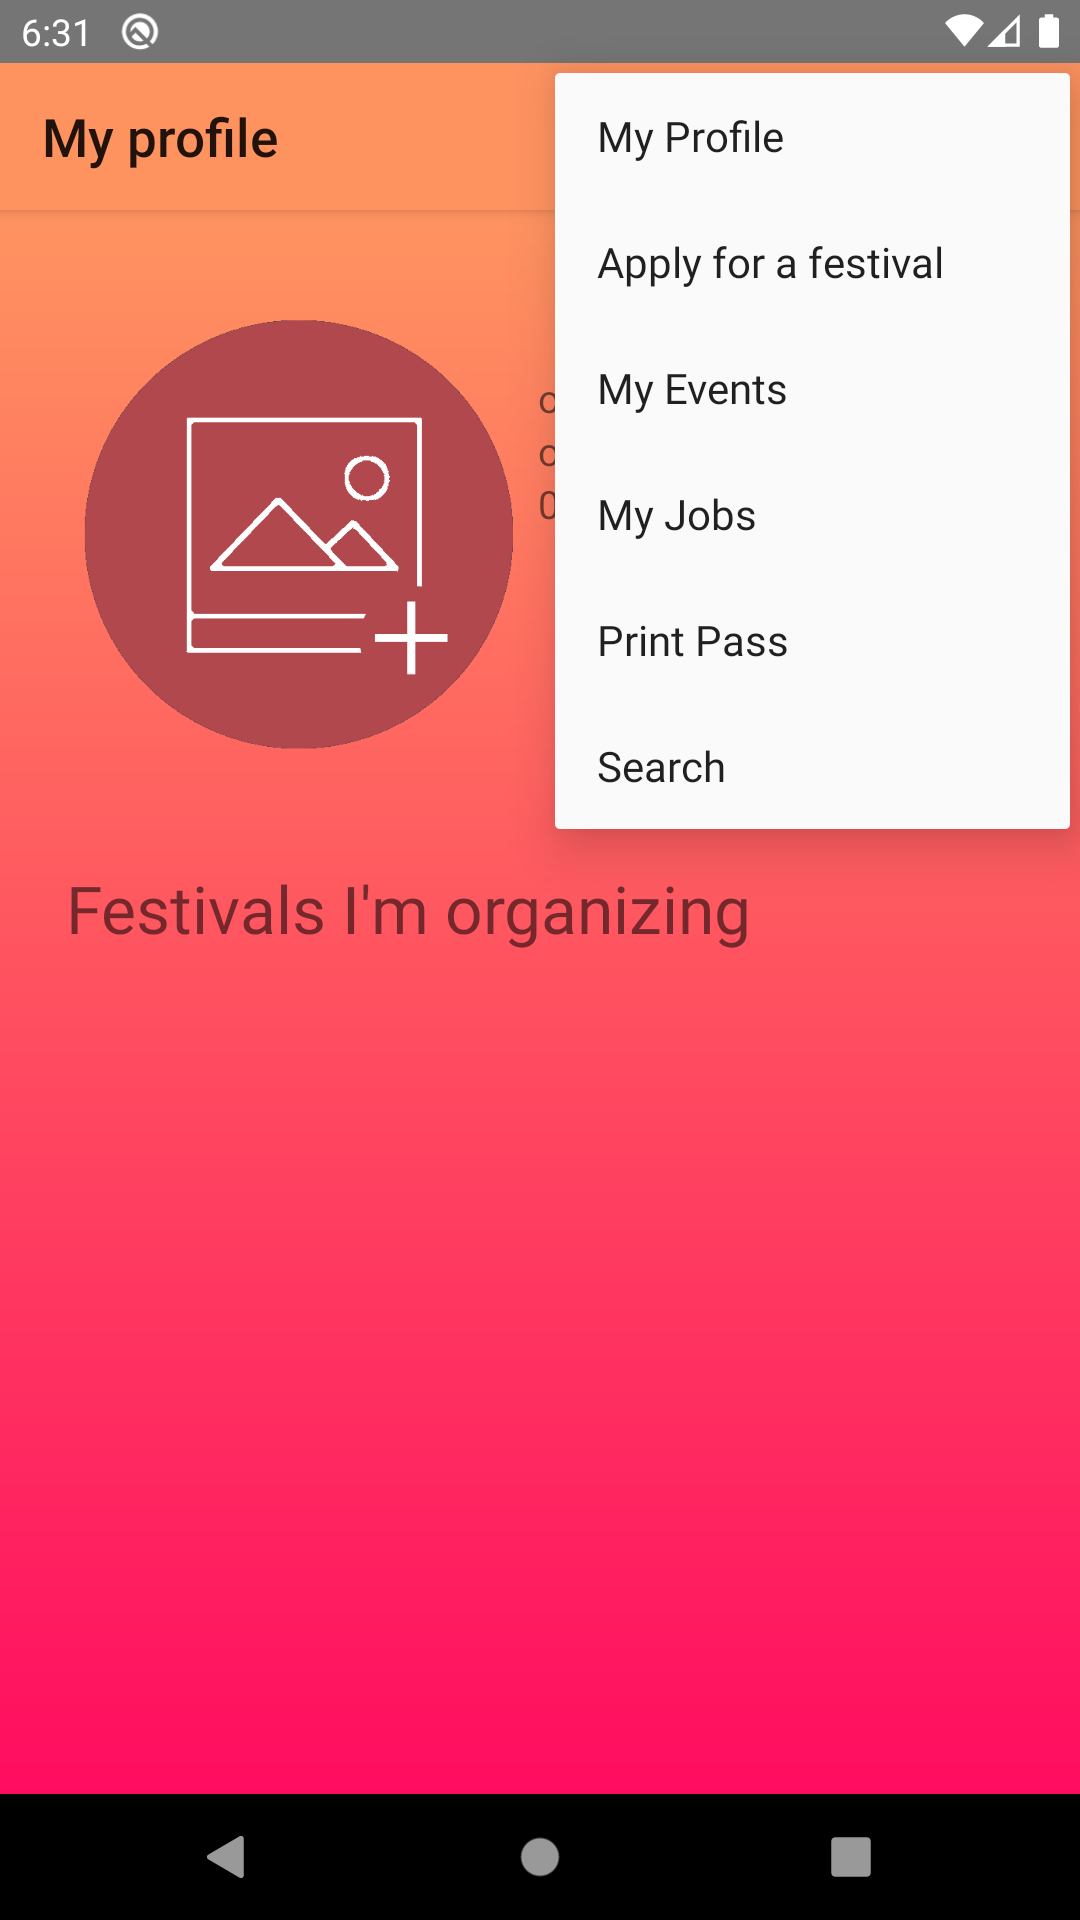
\includegraphics[width=\linewidth]{images/test_Screens/test_scenario_5-3.png}
				\caption{Test scenario 5}
				\label{fig:espresso_5_3}
			\end{figure}
	
			\begin{figure}[H]
				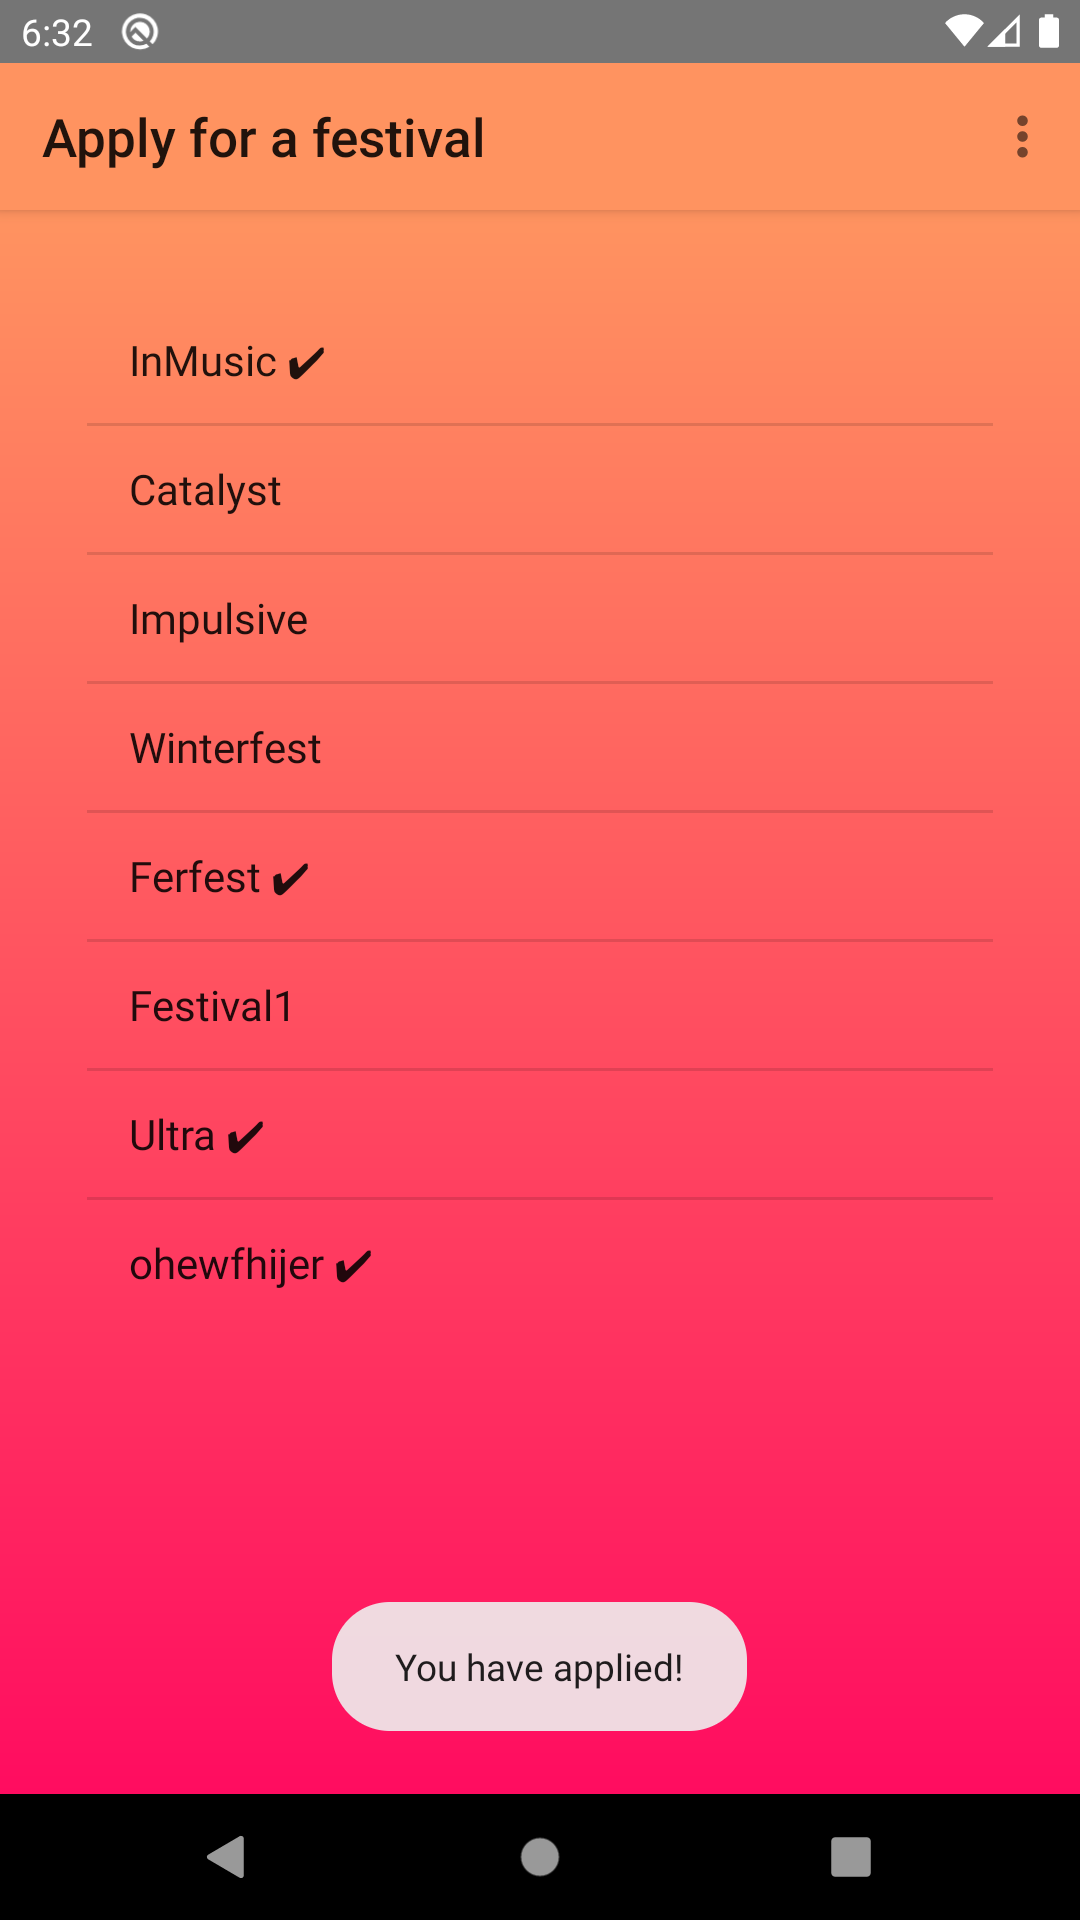
\includegraphics[width=\linewidth]{images/test_Screens/test_scenario_5-4.png}
				\caption{Test scenario 5}
				\label{fig:espresso_5_4}
			\end{figure}
			
			\textbf{Test scenario 6 - Worker multiple tests}
			Input:
			\begin{packed_enum}
				\item Input worker user data, tap 'Login'.
				\item Tap 'Add specialization'.
				\item Input new specialization and tap 'Add specialization'.
				\item Tap one specialization from list.
				\item Tap 'Apply for a job', tap one job from list, tap 'Apply', input data, tap 'Apply'.
				\item Tap back button, tap 'My applications', and tap one from list.
				\item Tap 'Search', input 'Marko', tap 'Search'.
				\item Tap 'Print Pass'.
				\item Tap 'Active jobs', tap 'My applications'
				\item Tap 'Log Out'.
			\end{packed_enum}
			
			Expected output:
			\begin{packed_enum}
				\item Login as worker.
				\item Opened specialization screen.
				\item Added new specialization on a list.
				\item Get message about successfully added specialization, see tick next to chosen specialization.
				\item Get message about successfully applied for a job.
				\item See data about chosen application.
				\item See results from search for 'Marko'.
				\item Get message about successfully created PDF file with pass, and get file created in storage.
				\item See 'Active jobs' screen, see 'My application' screen.
				\item Log out, and see login screen.
			\end{packed_enum}
			
			Actual result:
			\begin{packed_enum}
				\item Login as worker.
				\item Opened specialization screen.
				\item Added new specialization on a list.
				\item 'Randomly' chosen specialization and tick next to that randomly chosen specialization. (BUG shown)
				\item Get message about successfully applied for a job.
				\item See data about chosen application.
				\item See results from search for 'Marko'.
				\item Get message about successfully created PDF file with pass, and get file created in storage.
				\item See 'Active jobs' screen, see 'My application' screen.
				\item Log out, and see login screen.
			\end{packed_enum}
		
			\textbf{Test Scenario 7 - Admin accept leader test}
			Input:
			\begin{packed_enum}
				\item Input admin user data, tap 'Login'.
				\item Accept one leader from list of pending leaders.
			\end{packed_enum}
			
			Expected output:
			\begin{packed_enum}
				\item Login as 'admin'.
				\item Get message about successfully accepted leader.
			\end{packed_enum}
			
			Actual result:
			\begin{packed_enum}
				\item Login as 'admin'.
				\item Get message about successfully accepted leader.
			\end{packed_enum}
		
			\eject
		\section{UML Deployment Diagram}
		
			Due to the application including a lot of users, we have opted for the specification deployment diagram.
			The application consists of two parts: the mobile application(kind of a front-end) and the back-end hosted on the Pythonanywhere cloud. The application uses protocols GET(for information retrieval from the server), and POST in order to send/communicate information to the server. Furthermore, the server consists of 4 parts:
			\begin{itemize}
				\item App.db - definition of the database for SQLite 3
				\item Models.py - database tables modelled as Python classes
				\item Run.py - endpoint initialisation and control
				\item Resource.py - Used for handling server requests and responses
			\end{itemize}
			
			As far as hardware goes - basically 2 devices are required - the mobile phone and the cloud hosting computer. Network is also required as it is used to convey
			information between these 2 endpoints. While there is only one server instance, it is expected that multiple concurrent mobile phones will be using the application. Therefore, in the instance deployment diagram more than one mobile phone could be present.
		
			\begin{figure}[H]
				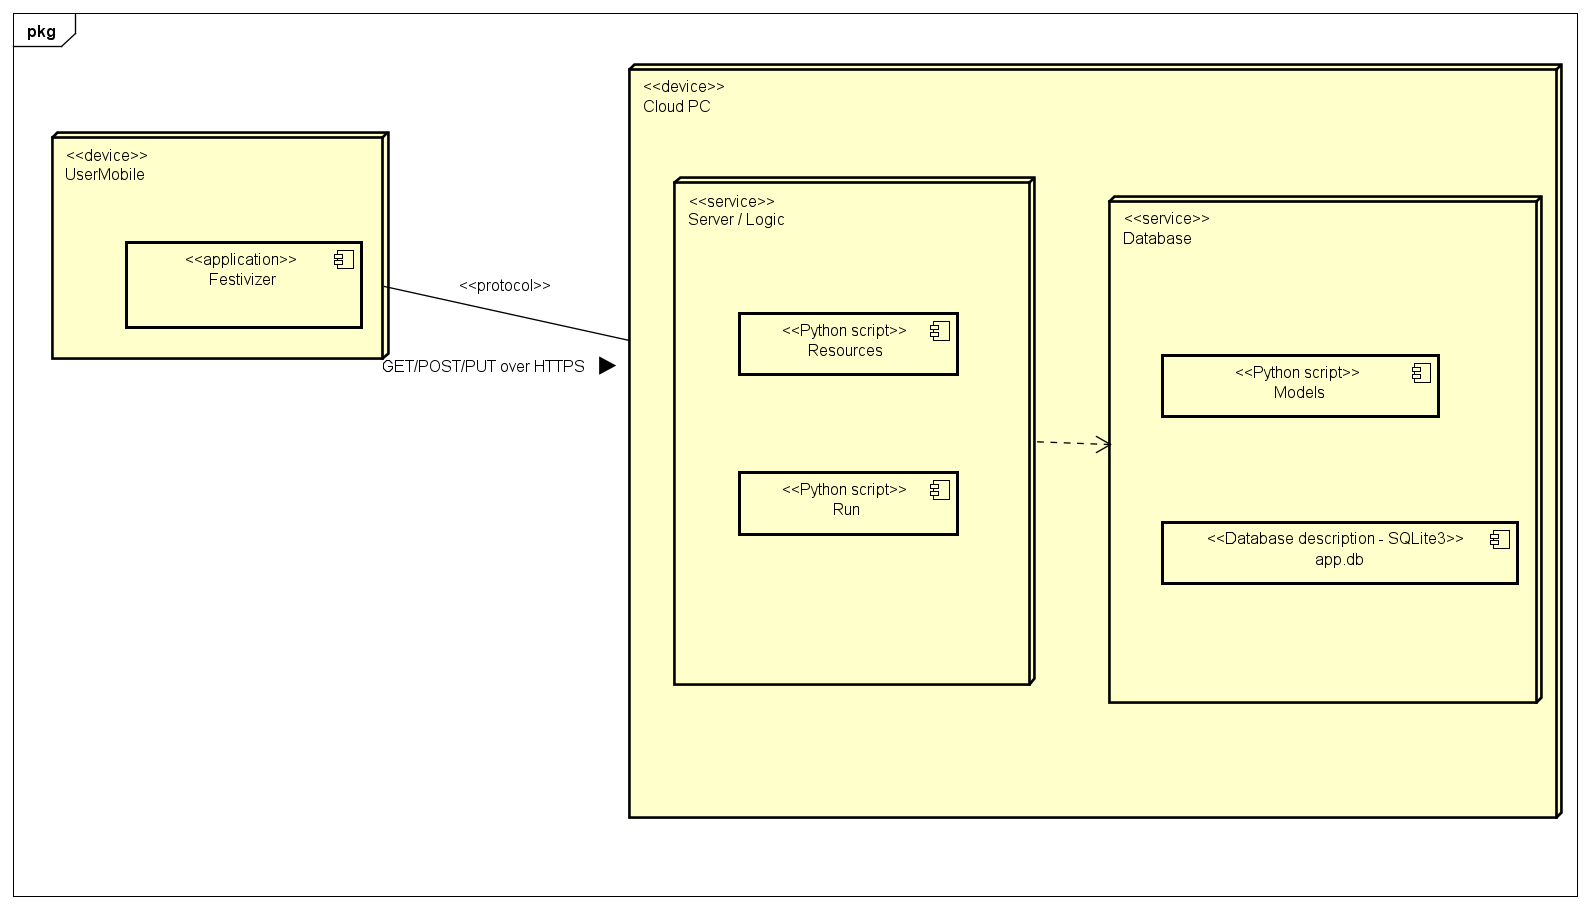
\includegraphics[width=\linewidth]{diagrams/Deployment Diagram0.png}
				\caption{Deployment Diagram}
				\label{fig:deployment_diag}
			\end{figure}
		
			\eject			
		\section{Deployment instructions}
			
			\subsection{Building the APK}
			
			The APK can be built in the following way:
			First, you need to git clone the application's repository: \href{https://gitlab.com/barbil/organization_of_the_festival}{The git repository}
			
			\begin{figure}[H]
				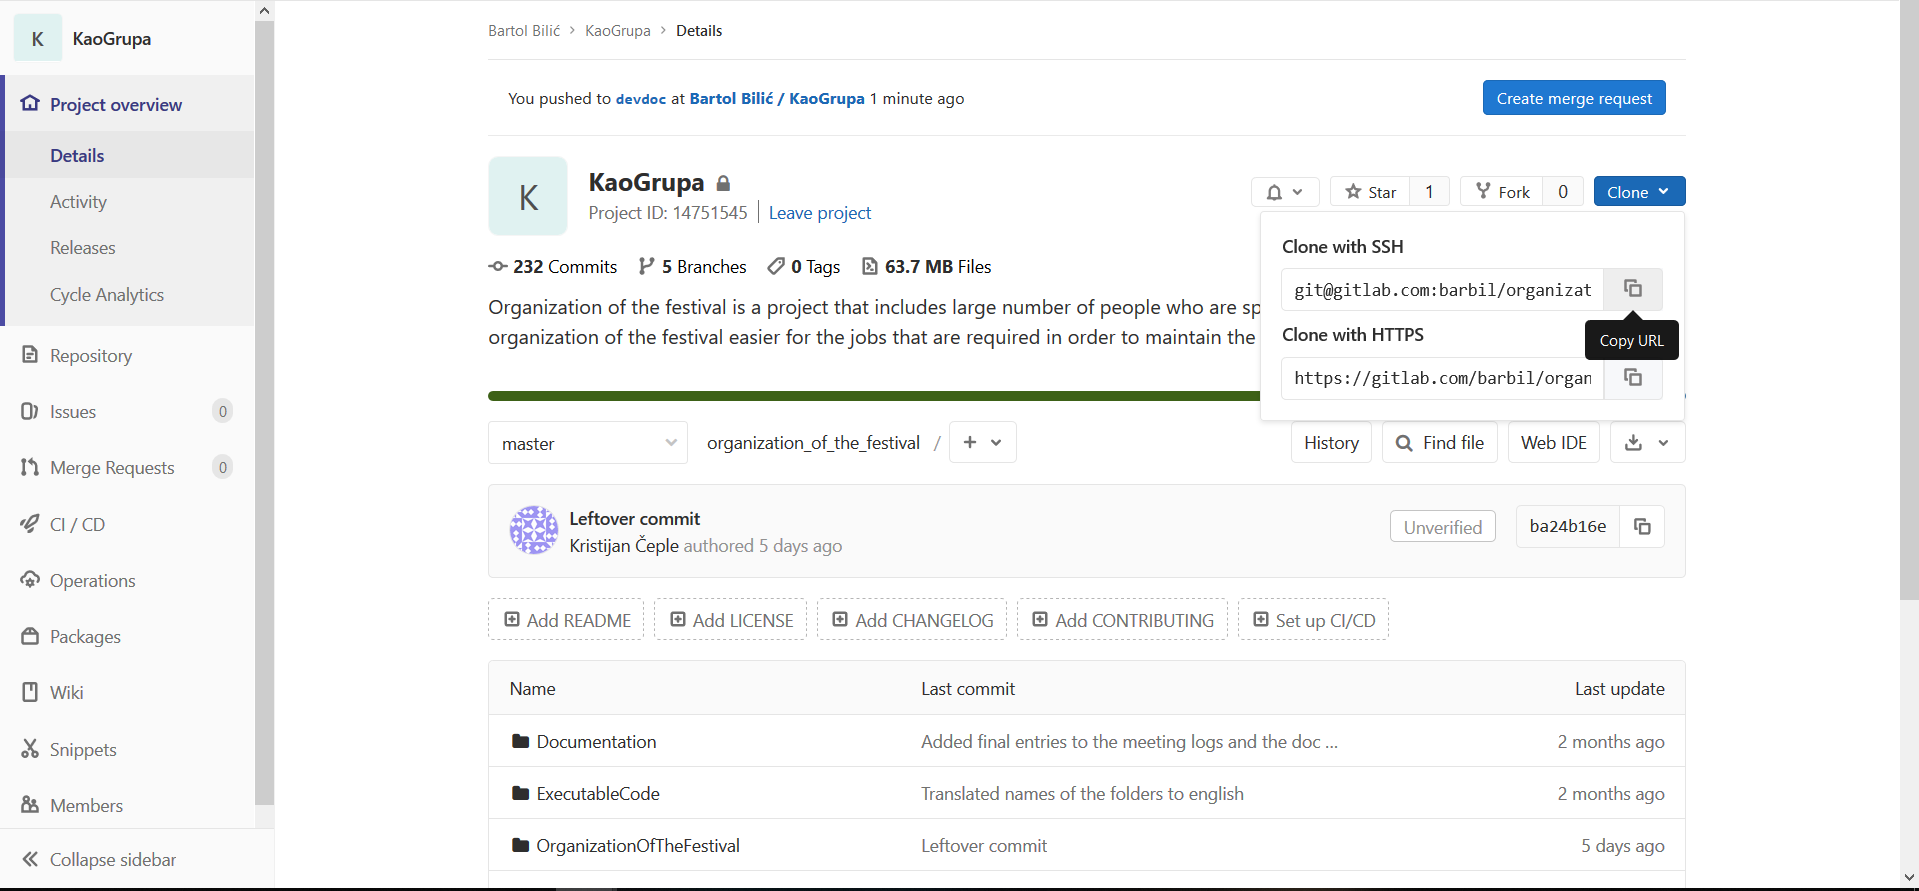
\includegraphics[width=\linewidth]{images/Deploy_M_1.png}
				\caption{Cloning from git}
				\label{fig:install_1}
			\end{figure}
			
			After pulling, the project needs to be opened in Android Studio. Merely go \textbf{File -> Open}, and then navigate to the cloned git repository. There you will find the project file that can be opened. Now, you would want to build an APK to run it on your device.
			
			\begin{figure}[H]
				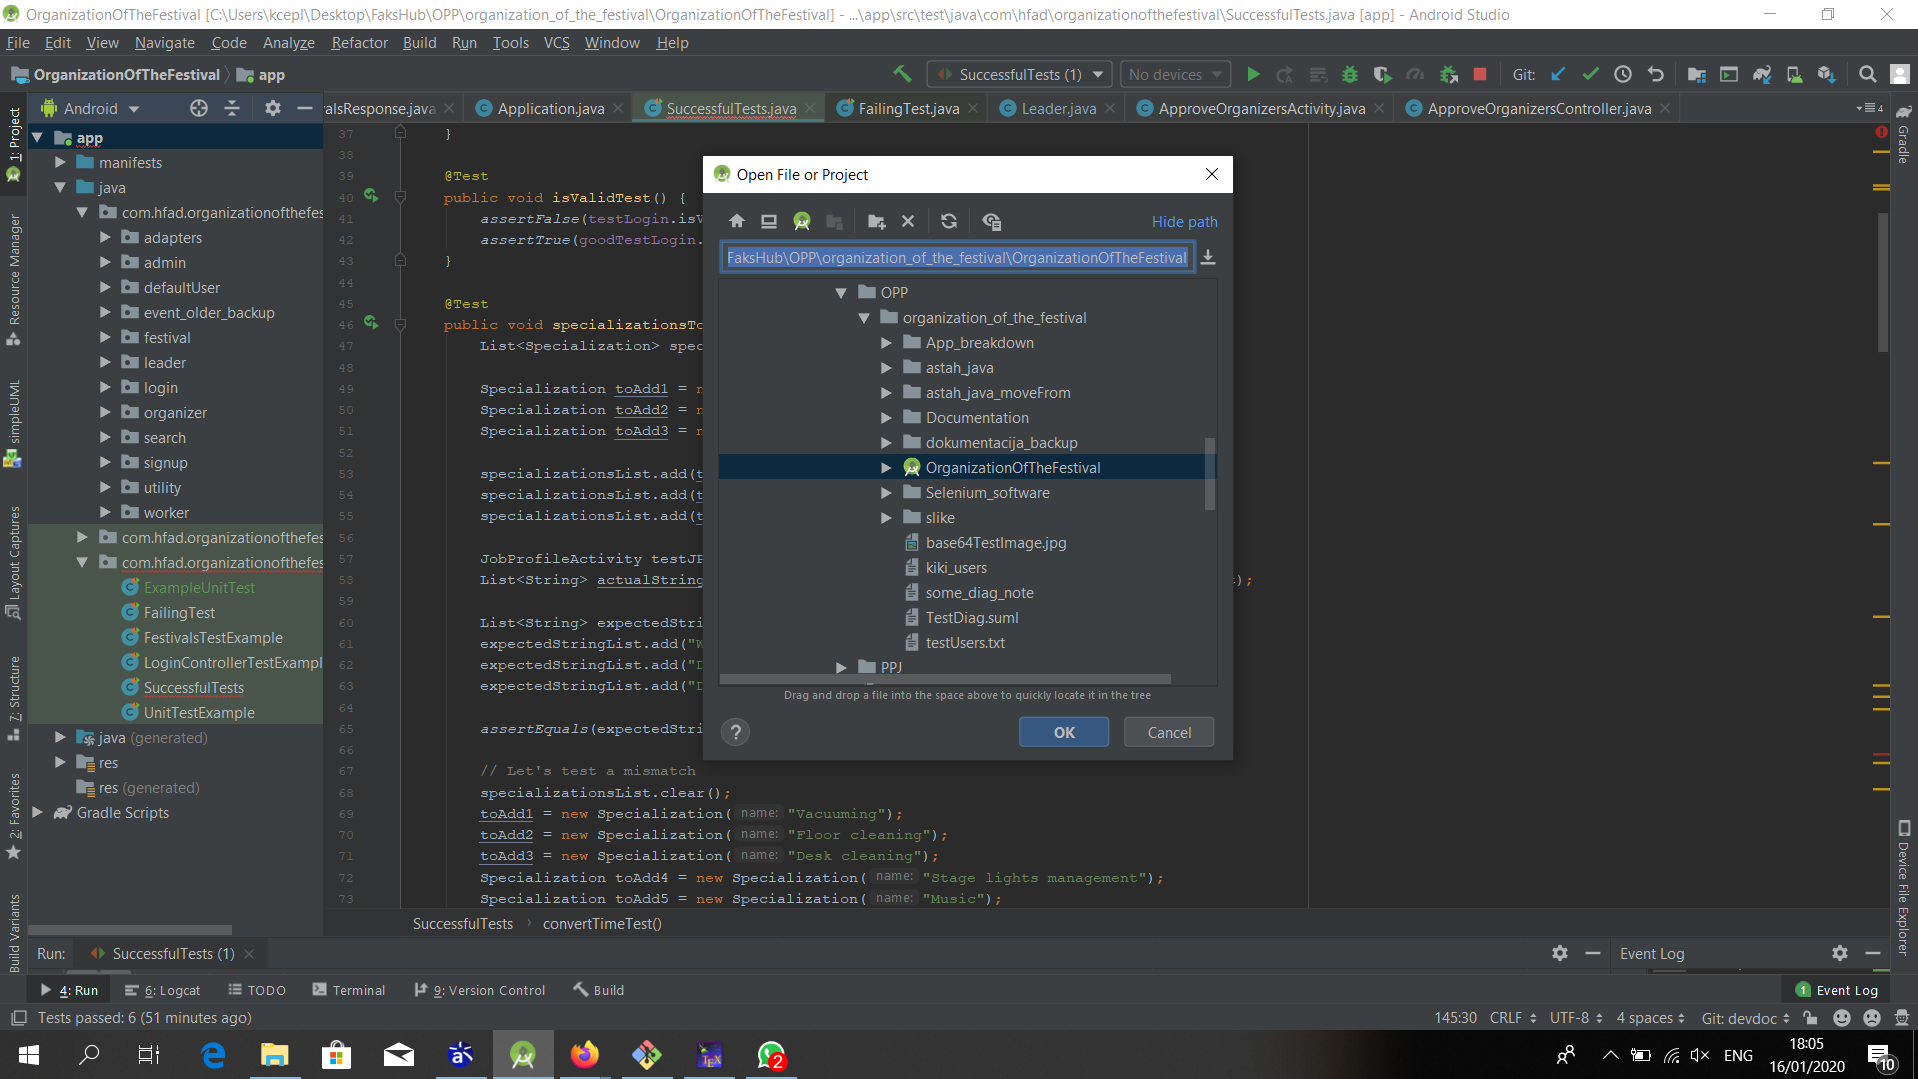
\includegraphics[width=\linewidth]{images/Deploy_M_2.png}
				\caption{Opening the Project}
				\label{fig:install_2}
			\end{figure}
			
			There is also an alternative. It is to go to our store, and install the app from there. Also, it is possible to build a signed build in Android Studio that is ready for deployment on any App store. Link of our application: \href{https://play.google.com/store/apps/details?id=com.hfad.organizationofthefestival}{App Store entry}
			
			Here, we will go into the process of generating your APK. Go to \textbf{Build -> Build Bundle(s)/APK(s)} or \textbf{Build -> Build Signed Bundle/APK}. If opting for signed bundles and APKs, you will need to generate a secure key that will be used for the signing process.
			
			\begin{figure}[H]
				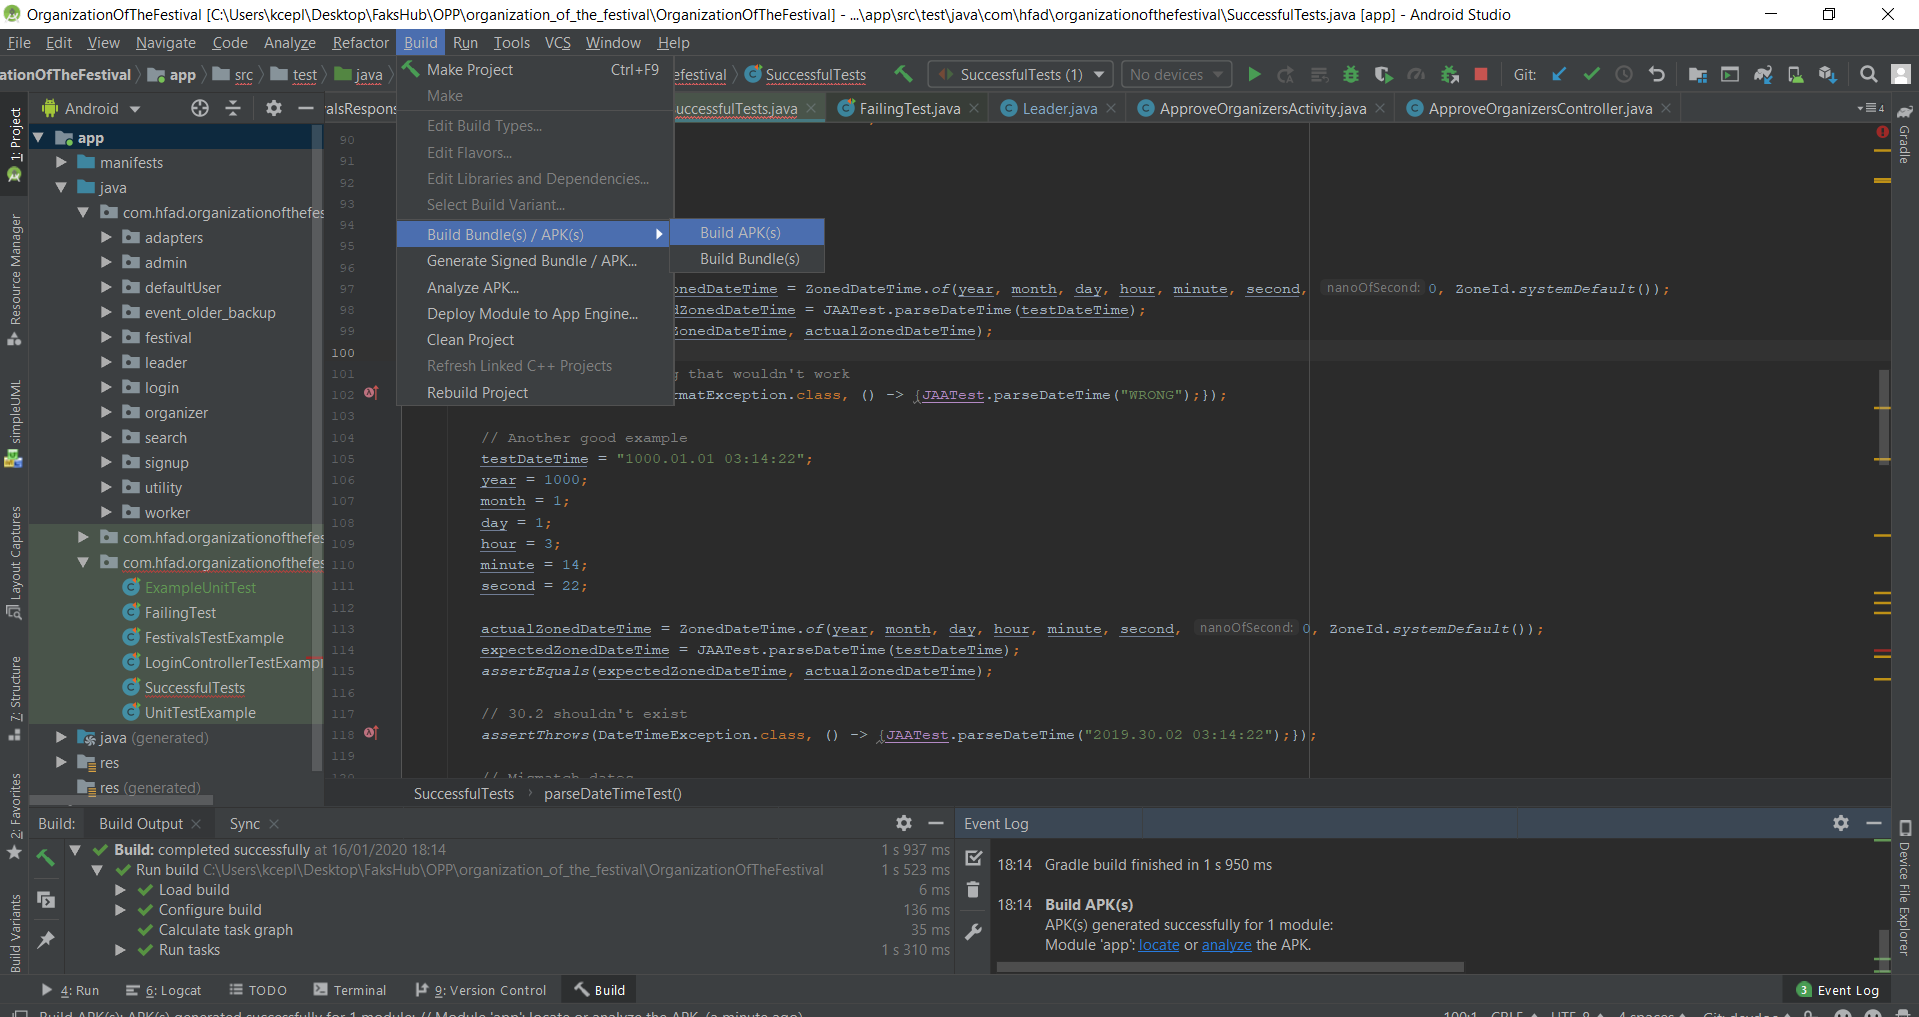
\includegraphics[width=\linewidth]{images/Deploy_M_3.png}
				\caption{Building process}
				\label{fig:install_3}
			\end{figure}
			
			\begin{figure}[H]
				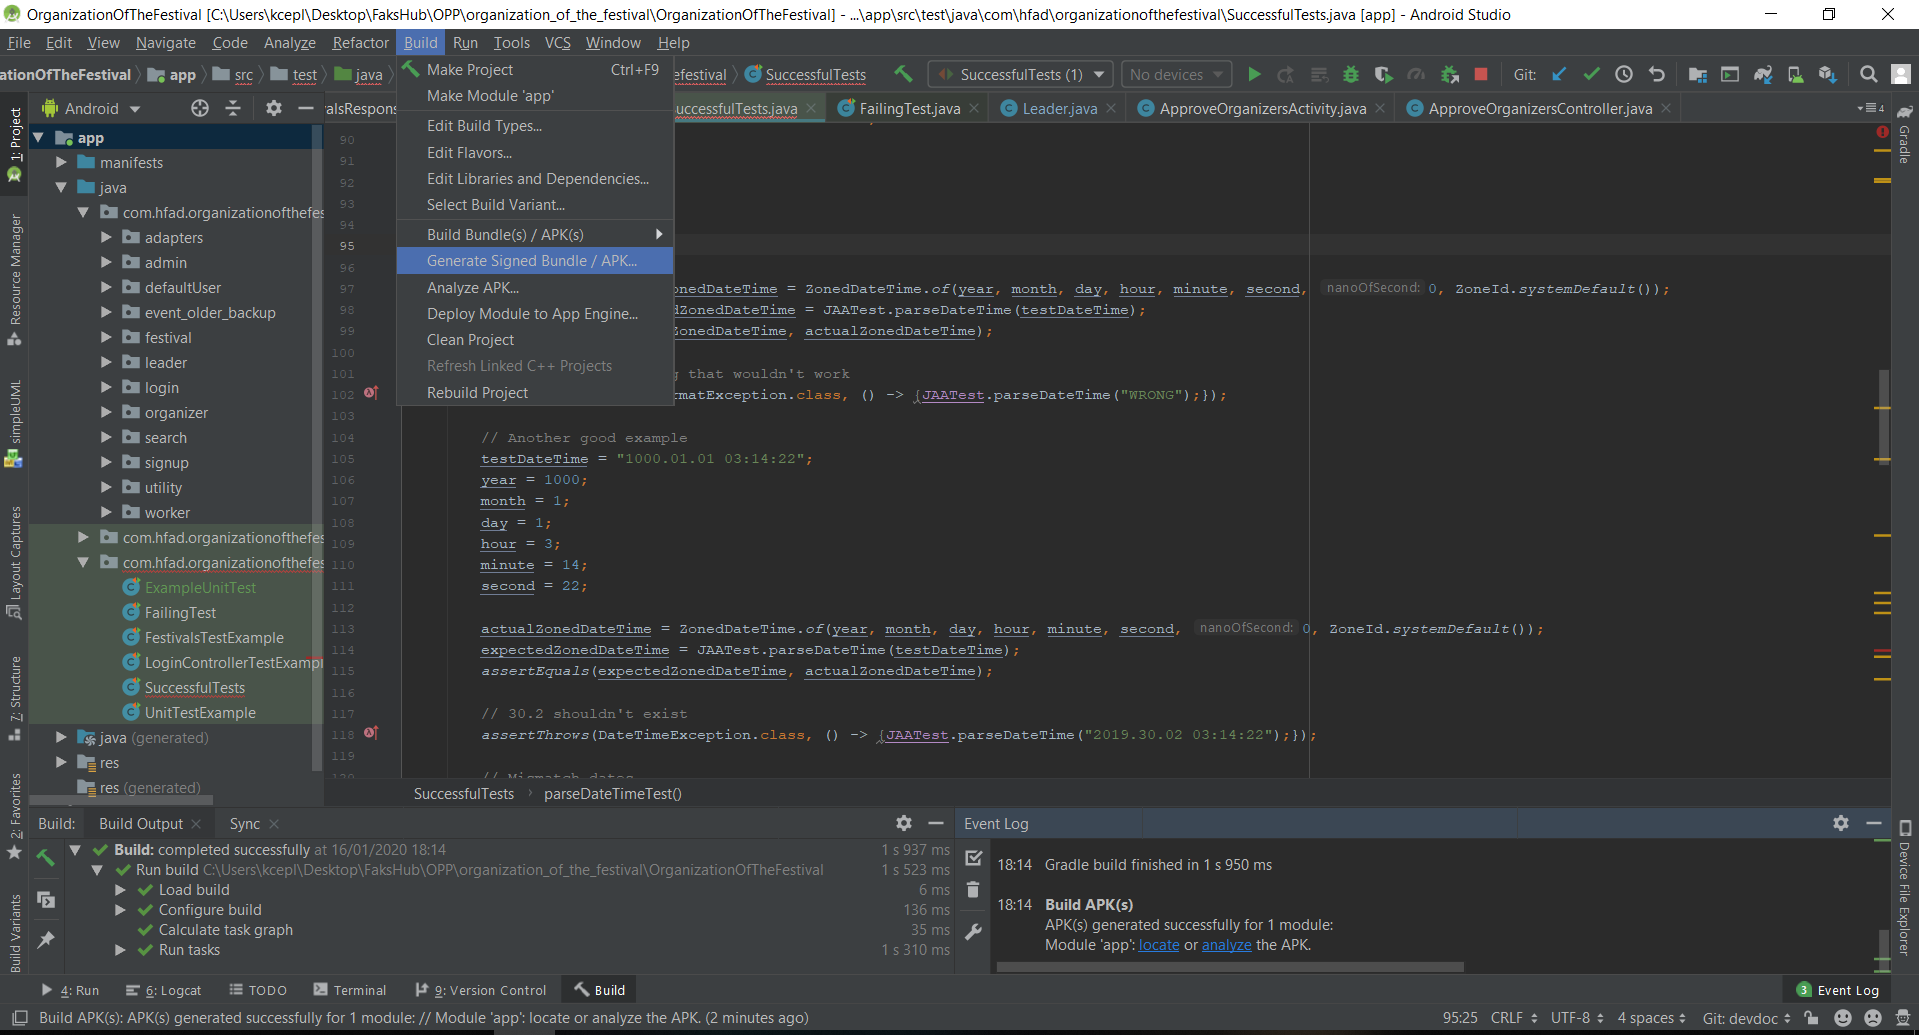
\includegraphics[width=\linewidth]{images/Deploy_M_4.png}
				\caption{Building process}
				\label{fig:install_4}
			\end{figure}
			
			\begin{figure}[H]
				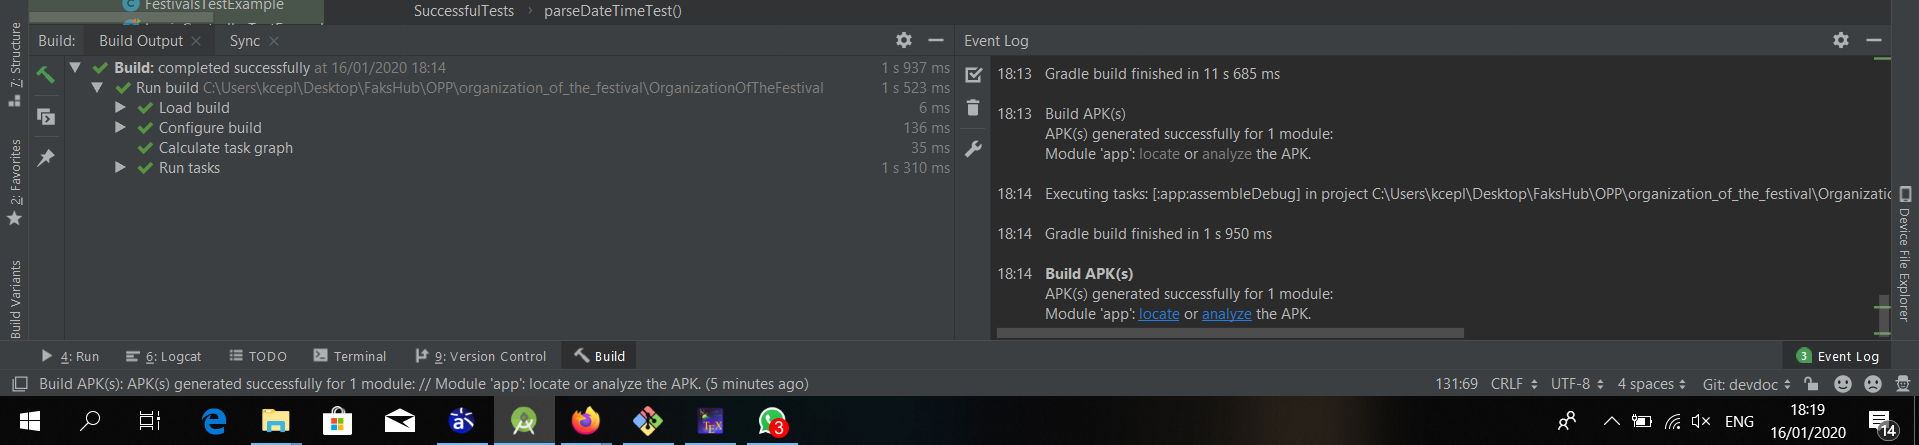
\includegraphics[width=\linewidth]{images/Deploy_M_5.png}
				\caption{Building process}
				\label{fig:install_5}
			\end{figure}
			
			Once you have the APK, it can be uploaded to any app store. \textbf{The APKs that will be uploaded to the app store SHOULD be signed.} It is also possible to put this .apk on the mobile device, and install it it there.
			
			Upon running the application, it will automatically connect to the kaogrupa pythonanywhere site, and communicate with the server. You are now ready to use the application.
			
			\subsection{Setting up the server side}
				
				The files are already present on the git URI, branch server: \href{https://gitlab.com/barbil/organization_of_the_festival/tree/server}{The server branch}. First of all this git should be cloned down somewhere. The files inside will be put onto the server. For deployment we used pythonanywhere as a cloud site, since it allows easy and seamless deployment of Flask applications.
				
				Second of all, you should either register or log in into pythonanywhere site.
				\begin{figure}[H]
					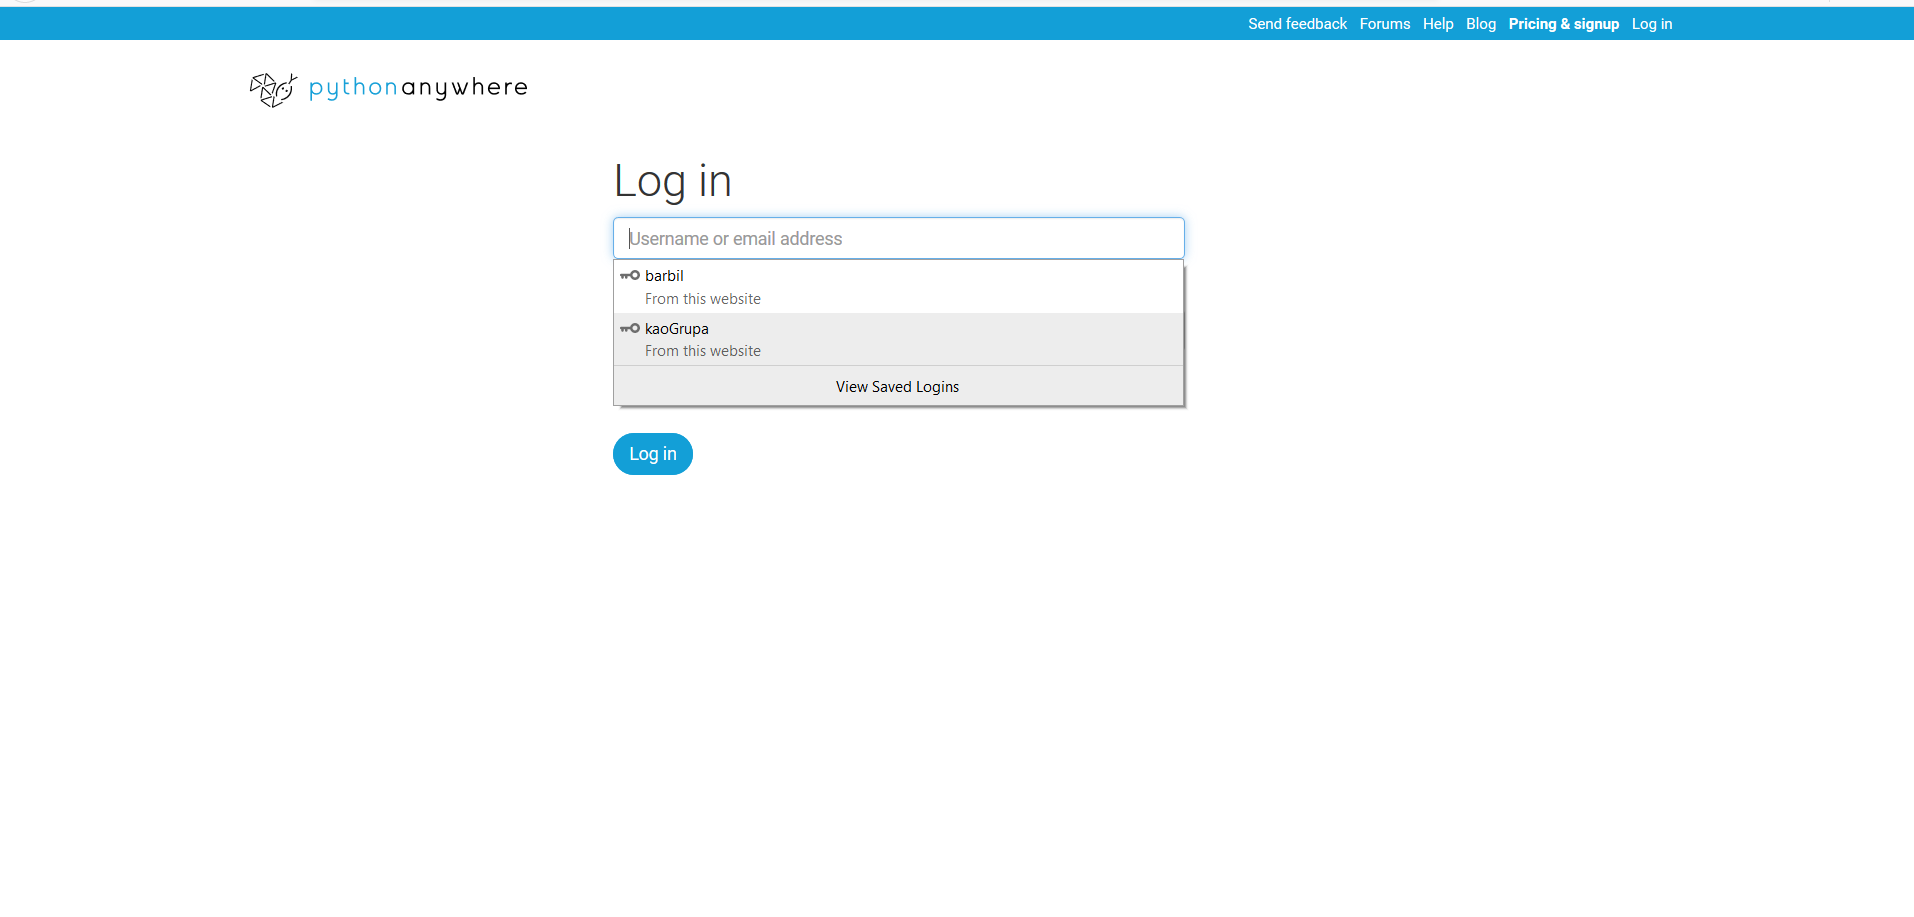
\includegraphics[width=\linewidth]{images/Deploy_1.png}
					\caption{Logging-In}
					\label{fig:deployment_1}
				\end{figure}
			
				Afterwards you should be taken to the dashboard screen. It should look something like this:
				\begin{figure}[H]
					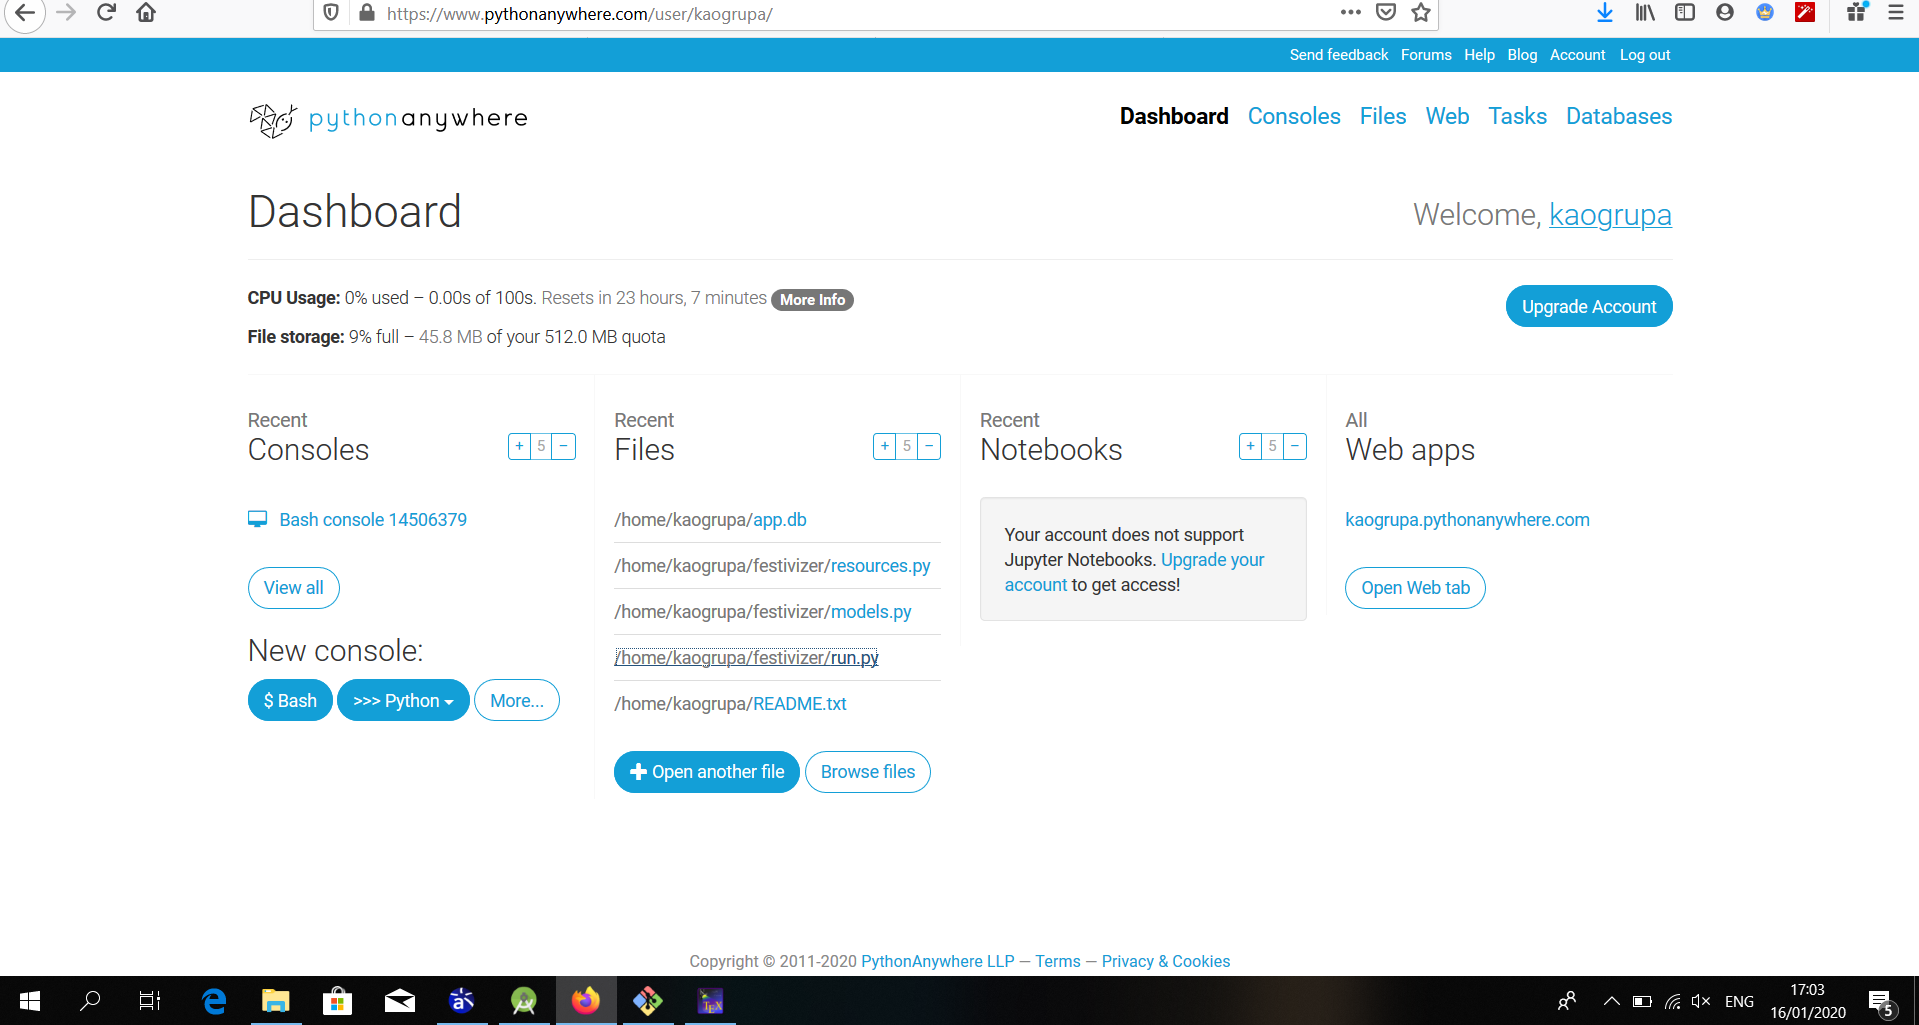
\includegraphics[width=\linewidth]{images/Deploy_2.png}
					\caption{Dashboard}
					\label{fig:deployment_2}
				\end{figure}
				
				Then click on the 'Open Web tab' button under the 'Web apps' title. Once there, click on the 'Add a new Web App' button.
				\begin{figure}[H]
					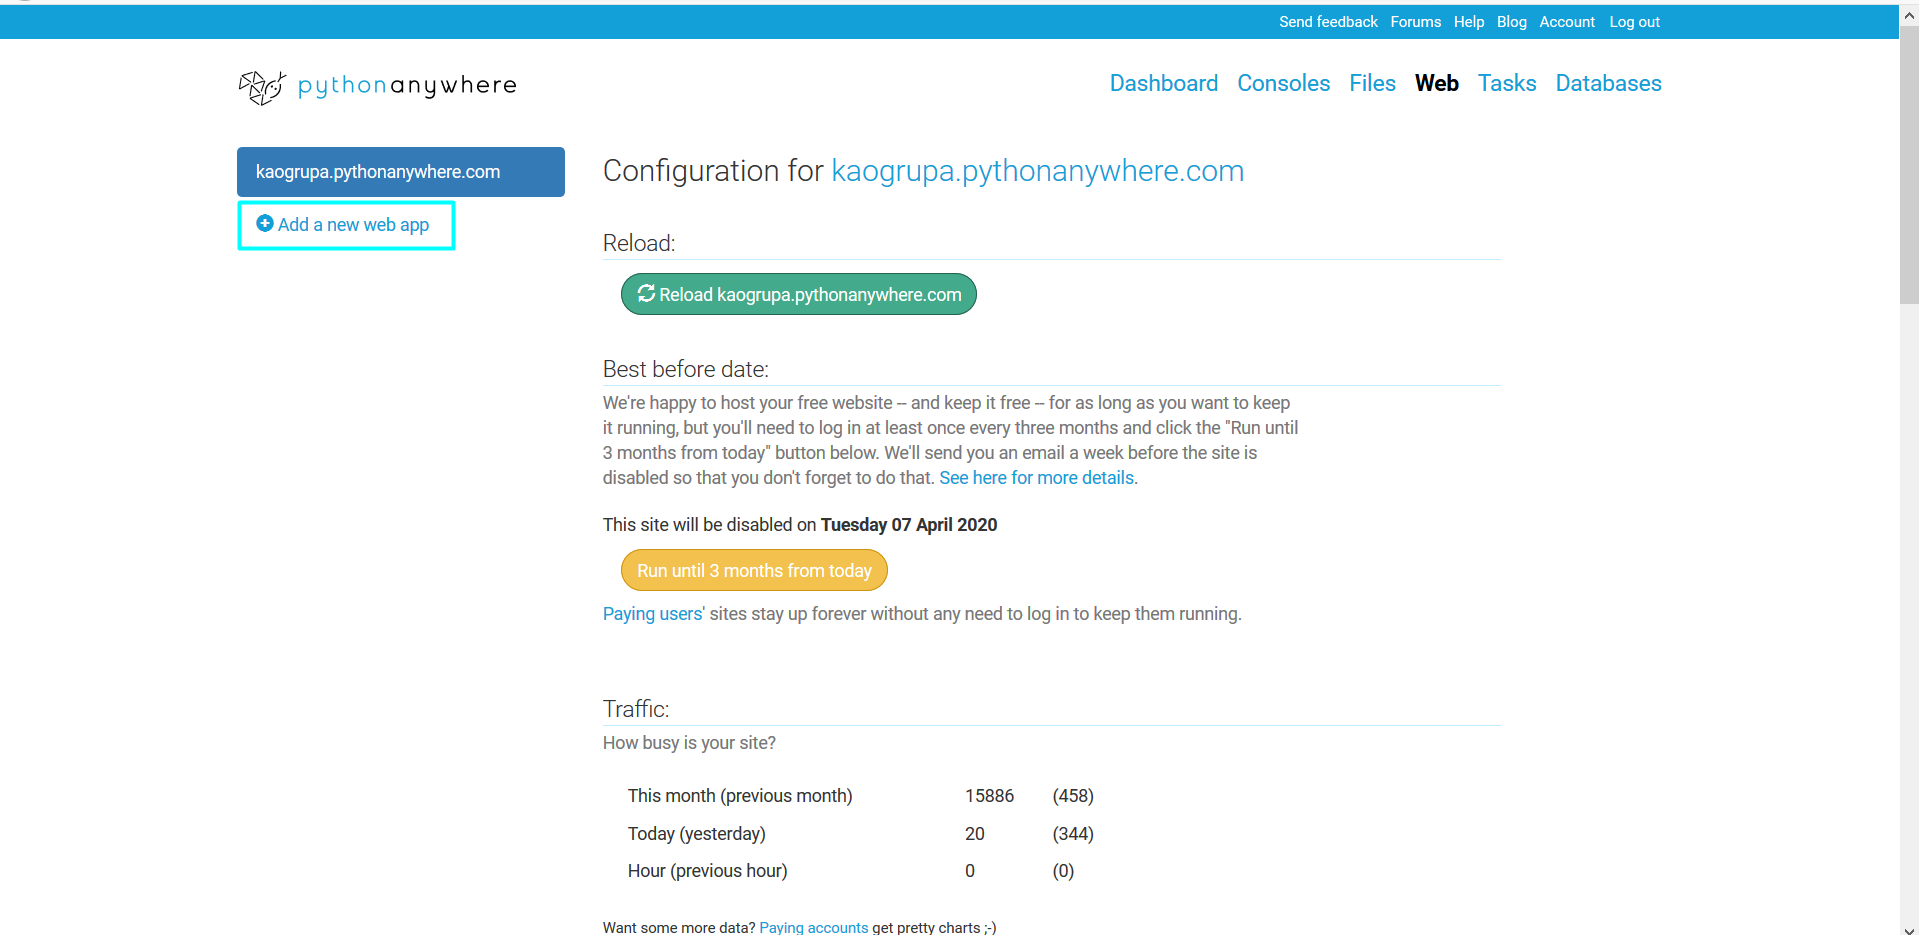
\includegraphics[width=\linewidth]{images/Deploy_3.png}
					\caption{Adding a new Web App}
					\label{fig:deployment_3}
				\end{figure}
				
				A wizard will appear on the right side, where you should select Flask. Python 3.6 is the minimum supported Python version. The default file flask\_app.py will be generated. 
				
				Now the project is set up. All that is needed is to upload the files. Flask\_app.py entry point file - you should put into it the app.py code from git. Also upload the other files to the server. You should now be set up - all that is left to do is to change the hardcoded kaogrupa URL in the application to point to your server. Once that is done, you have got your own back-end set up, and can comfortably change and experiment on the application.
				
				That is depicted on thee pictures below:
				\begin{figure}[H]
					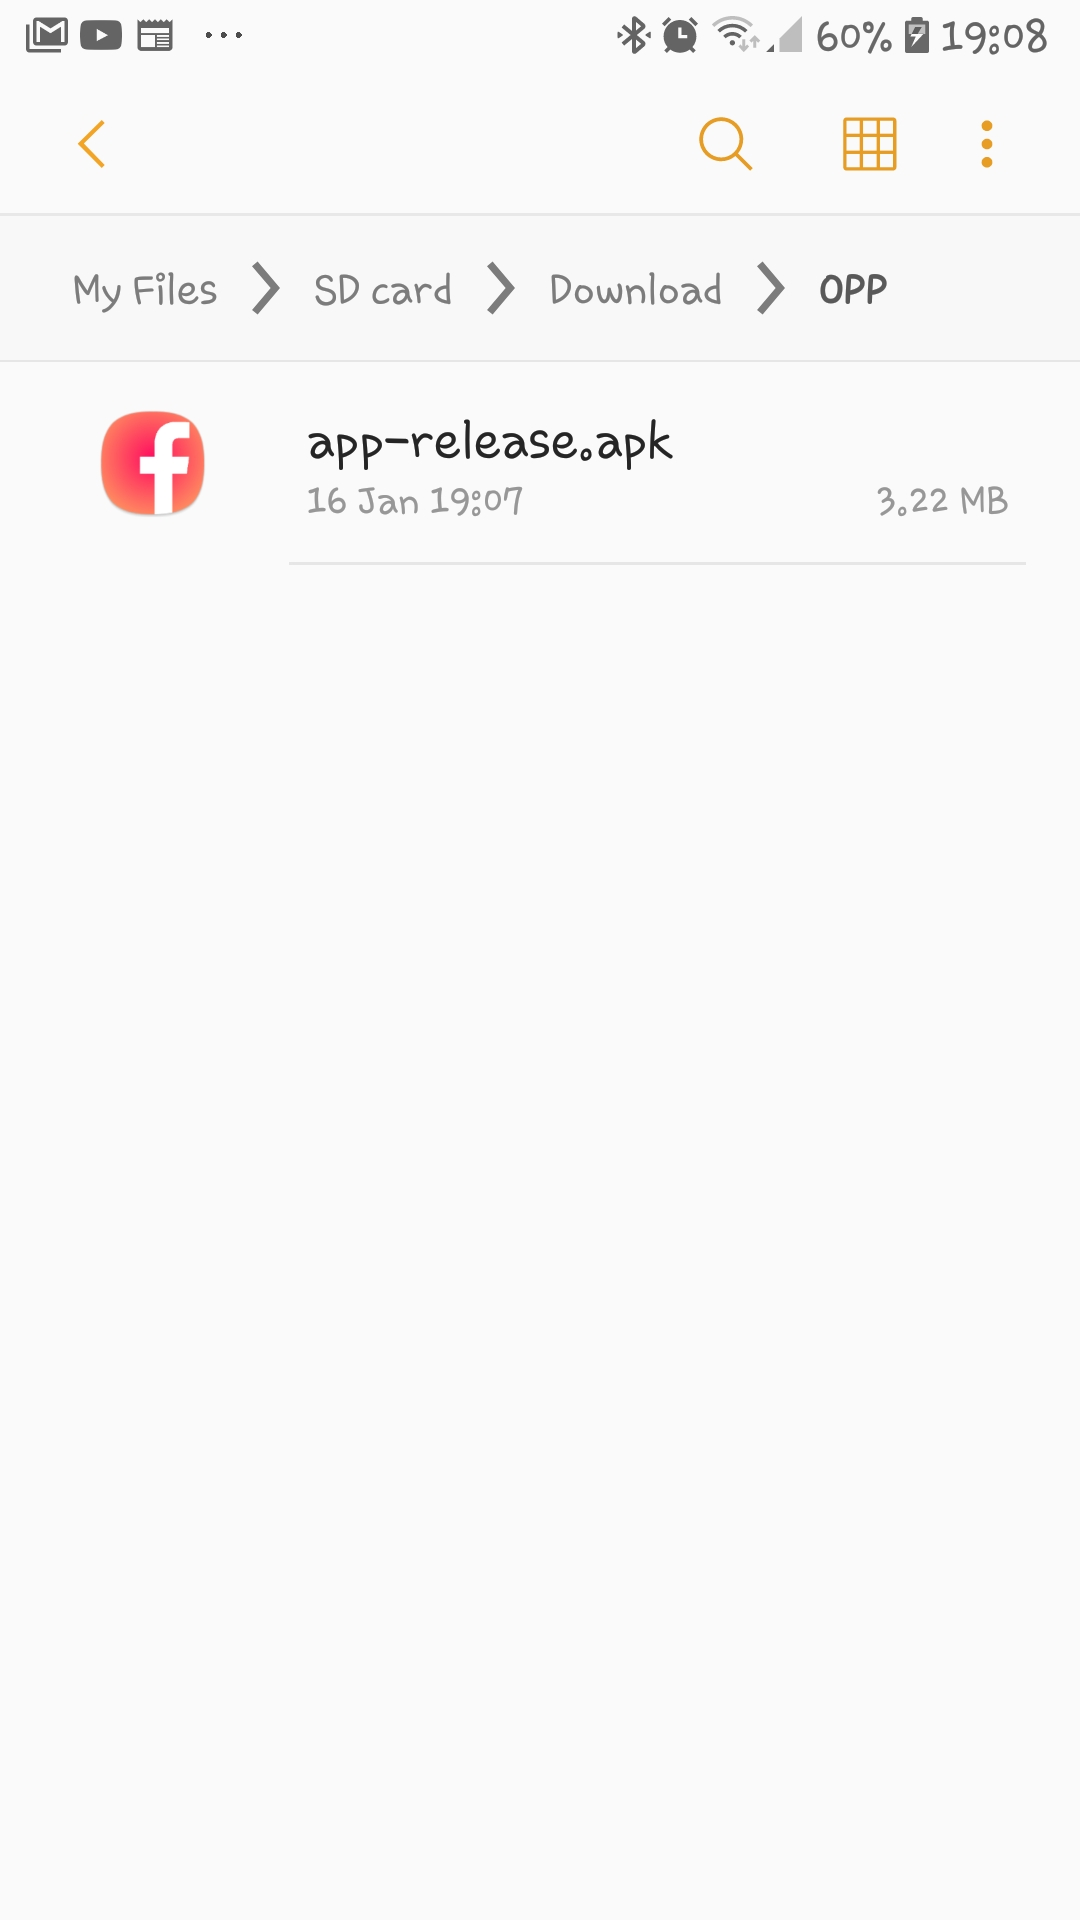
\includegraphics[width=\linewidth]{images/Android_1.jpg}
					\caption{Adding a new Web App}
					\label{fig:android_1}
				\end{figure}
			
				\begin{figure}[H]
					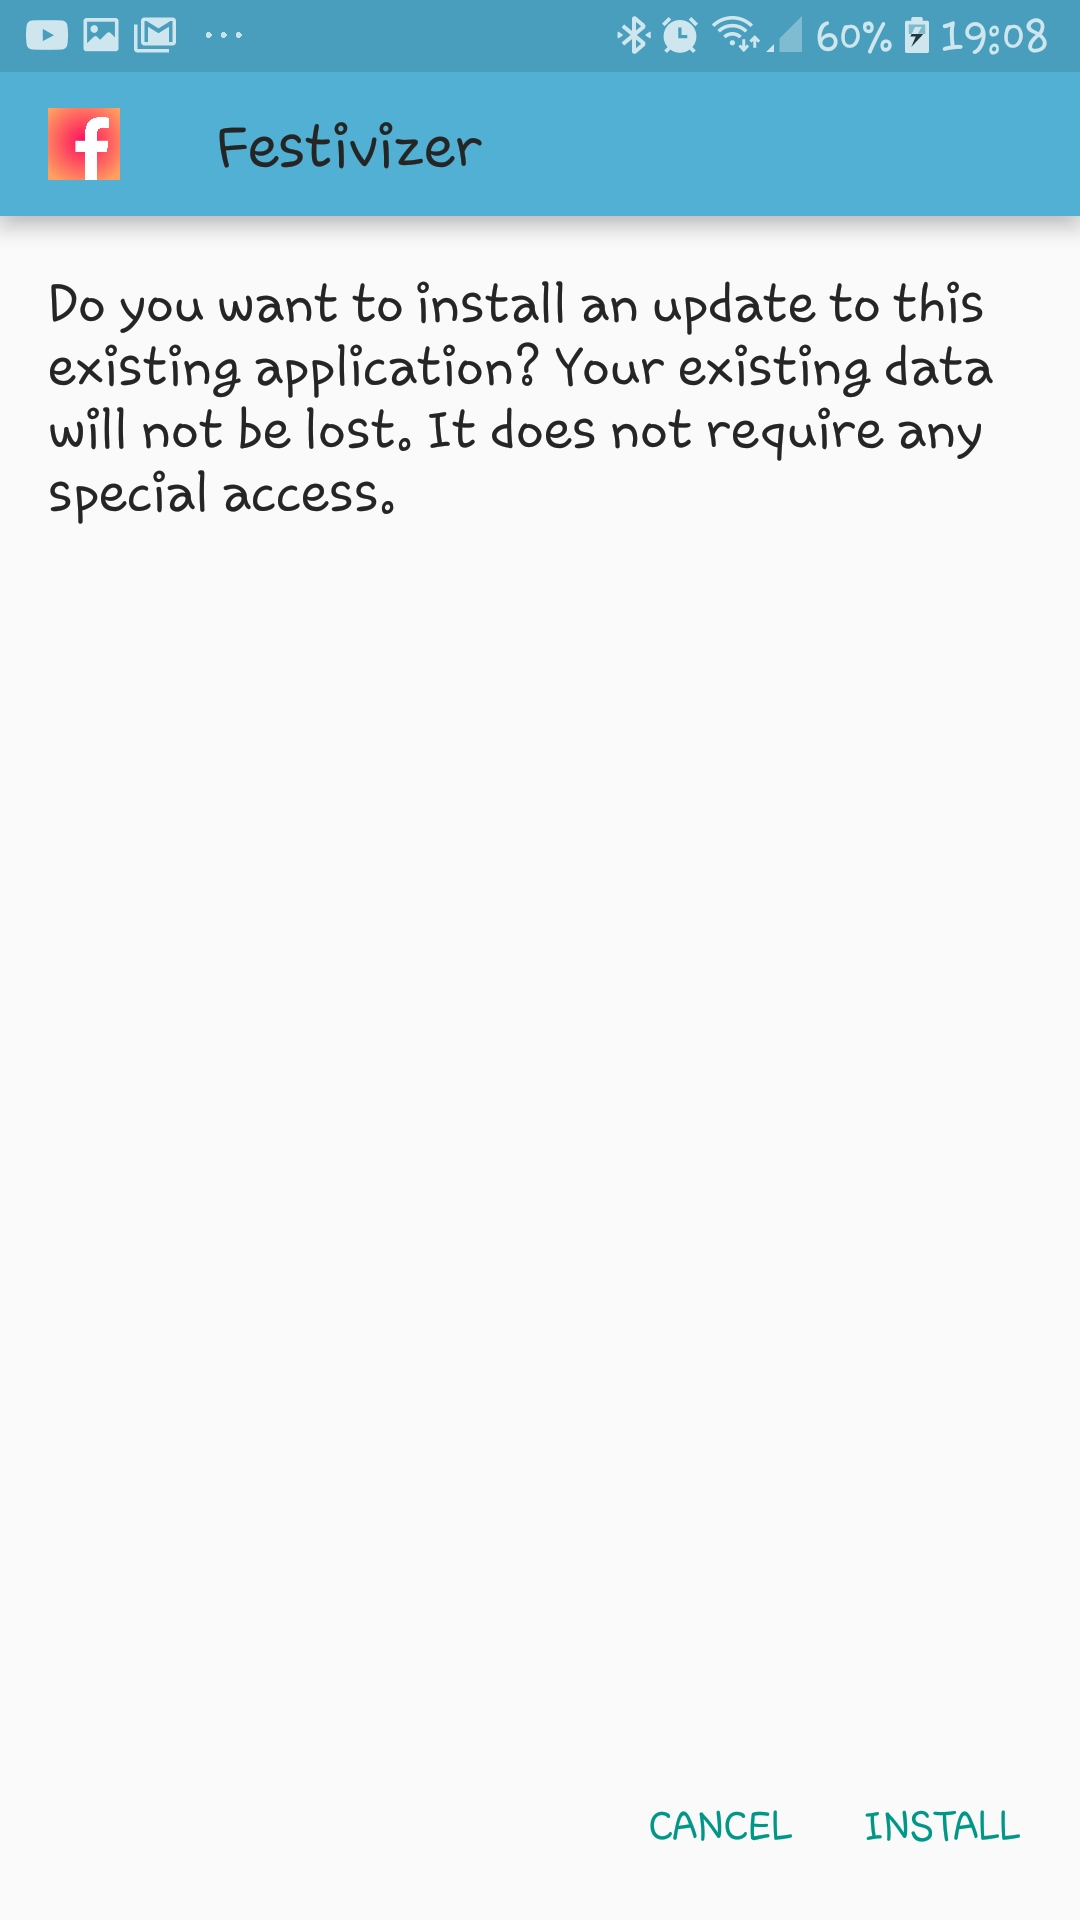
\includegraphics[width=\linewidth]{images/Android_2.jpg}
					\caption{Adding a new Web App}
					\label{fig:android_2}
				\end{figure}
			
				\begin{figure}[H]
					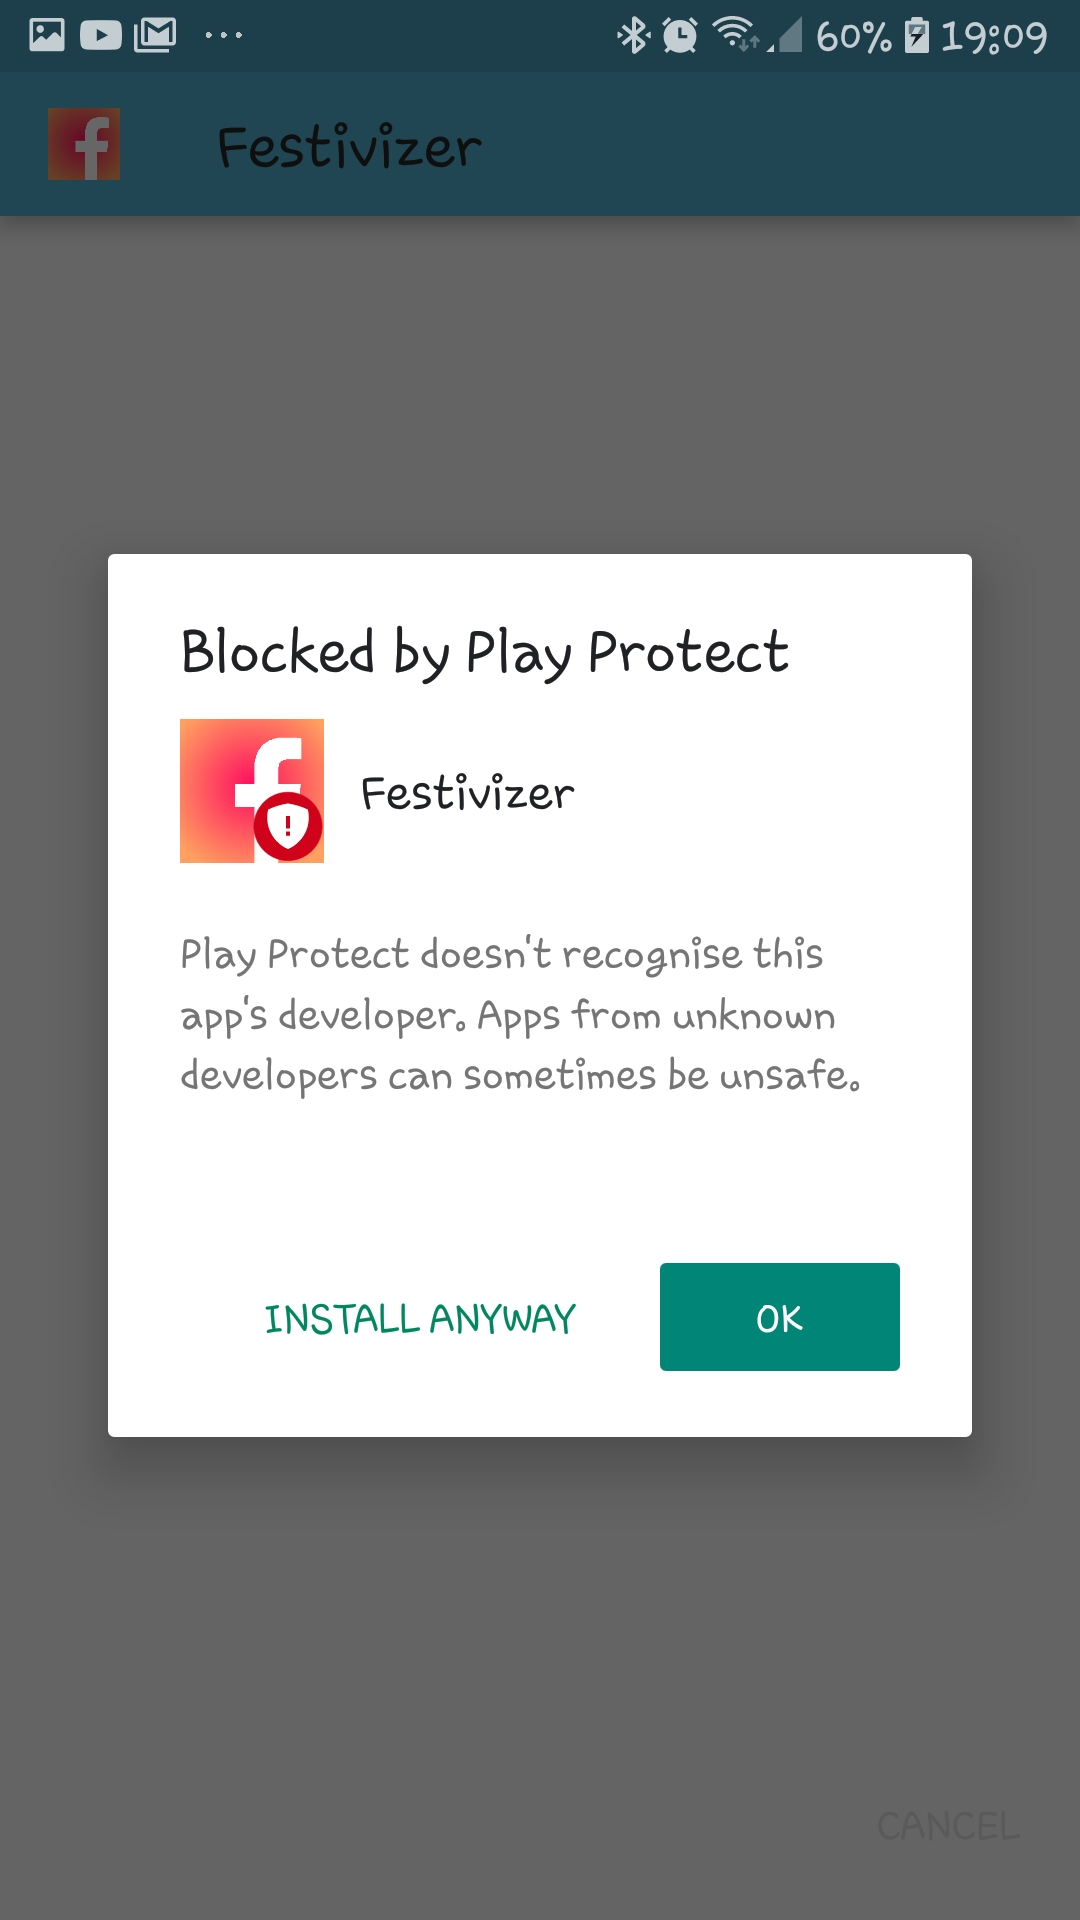
\includegraphics[width=\linewidth]{images/Android_3.jpg}
					\caption{Adding a new Web App}
					\label{fig:android_3}
				\end{figure}
			
			\eject 